\documentclass[11pt]{article}
\usepackage[margin=1in]{geometry}
\usepackage{amsmath,amssymb,amsthm,graphicx}
\usepackage[hidelinks]{hyperref}
\newtheorem{theorem}{Theorem}
\newtheorem{lemma}[theorem]{Lemma}
\newtheorem{proposition}[theorem]{Proposition}
\newcommand{\norm}[1]{\left\|#1\right\|}
\newcommand{\inner}[2]{\left\langle#1,#2\right\rangle}
\newcommand{\R}{\mathbb R}
\DeclareMathOperator{\artanh}{artanh}
\title{Two-Phase Certificate Bounds for Backtracking Frank--Wolfe\\
under Function-Dependent Curvature\\[3pt]\large Extended technical report}
\author{Yaroslav P. Lyakhov \and Stepan Suvorov}
\hypersetup{pdfauthor={Yaroslav P. Lyakhov and Stepan Suvorov}}
\date{15 October 2026}

\begin{document}
\maketitle
\begin{abstract}
We consider convex minimization over a compact convex set with a linear
minimization oracle and curvature bounded by
$\norm{\nabla^2 f(x)}\le H_0+H_1(f(x)-f_Q^*)$.
The optimal value is unavailable to the algorithm. We use accumulated
linear lower bounds to construct a computable upper certificate. Standard
quadratic backtracking attains certificate accuracy $\varepsilon$ in
$O(H_0D^2/\varepsilon+(1+H_1D^2)\log(U_0/\varepsilon))$ linear-oracle calls,
up to an explicit initialization term and the final verification call,
for $0<\varepsilon<U_0$. It requires no curvature or optimal-value input.
A phase argument bounds the cost of estimates that lag behind decreasing
local curvature. All function trials cost at most $1+2N$ plus an explicit
logarithmic overhead after $N$ updates. The same linear-oracle order holds
for two explicit steps, exact segment minimization, and a
certificate-scaled backtracking variant; normalization is not needed
for this order. For standard away-step backtracking, we extend the
certificate bound by counting atom removals. Under a geometric error
bound, a second phase estimate gives logarithmic
accuracy dependence and separates the $H_1$ warm-up term from the
$H_0$ logarithmic term, without parameter inputs. We also give a corrected
lower certificate for deterministically bounded oracle errors.
A local gap envelope removes strong convexity from the primal-to-certificate
conversion; strong convexity remains one sufficient condition for the
geometric error bound.
Experiments cover seven families, including real-data Poisson regression
with positive $H_1$. Controlled initialization, radius, and objective-unit
comparisons separate oracle budgets and reveal important baseline
sensitivities. A Poisson activity sweep excludes repeated starting
vertices from its primary summaries. Two further count datasets show
that online certificate attainment can lag the independently bounded
primal error. Causal block-averaged tangent controls do not yield earlier
stopping on these paths; a standard known-strong-convexity control
resolves much of the lag on one dataset, using additional information.
No uniform empirical superiority
of certificate initialization or priority over all adaptive analyses
is established.
Independent proof checking and a complete priority audit remain necessary.
\end{abstract}

\noindent\emph{Version scope.} This report preserves the expanded
derivations and historical studies. The companion focused
\texttt{article.pdf} contains the subsequent exact differential
gap envelope and the zero-base finite-termination theorem. Saved
experiment thresholds in this report retain their original definitions.

\section{Introduction and scope}
Frank--Wolfe methods replace projections by linear minimization over the
feasible region. The resulting oracle model is attractive when linear
minimization is inexpensive and sparse convex combinations are useful;
see the survey~\cite{braun}. A global smoothness constant can nevertheless
make a short step conservative. Function-dependent curvature offers a
different way to choose an explicit step.

The condition studied here is motivated by the loss-suboptimality curvature
model of Alimisis, Islamov, and Lucchi~\cite{warmup}. Related developments
include generalized-smooth clipped methods~\cite{lobanovkoloskova} and
accelerated full-gradient and coordinate methods~\cite{lobanov}.
Vyguzov and Stonyakin~\cite{vyguzov} analyze Frank--Wolfe with curvature
depending on the gradient norm, including adaptive parameter selection.
Other practical choices include backtracking~\cite{pedregosa}, secant
line search~\cite{hendrych}, and the recent auto-conditioned framework~\cite{autoconditioned}.
Analytic steps derived from other curvature
models also exist, for example generalized self-concordance~\cite{selfconcordant}.
Adaptive Bregman steps treat relative smoothness~\cite{bregmanfw}, while
adaptive conditional gradient sliding reuses gradients across inner
linear-oracle iterations~\cite{adcgs}. Their assumptions and oracle units
require a separate comparison; the present study does not establish
superiority over these broader frameworks.

Extended-curvature error-bound rates~\cite{wirth} and restart schemes
adaptive to error bounds~\cite{restartfw} further constrain any priority
claim. Linear objective- and FW-gap convergence beyond global gradient
smoothness also precedes this work for log-homogeneous barriers~\cite{zhao}.
Appendix~\ref{sec:prioranalysis} records the precise comparisons used here.

The candidate contribution is an analysis of standard FW and away-step
backtracking under
\eqref{eq:curvature}, with separate dependence on $H_0,H_1$, a computable
stopping criterion, an initialization term, and a bound on all function
trials. It is a result about an existing method; it does not require a
new step-size rule. The linear certificate, scalar
differential comparison, halving argument, quadratic acceptance test, and
telescoping count of failures are standard tools. The quadratic step has
the same guarantee as the hyperbolic step, as does classical exact line
search in the linear-oracle model. An elementary function in a step rule
is therefore not the main claim. We do not establish optimal oracle
complexity, an accelerated rate for all smooth functions, or priority over
all adaptive analyses. The related-work search in this working version is
targeted and incomplete.

\section{Setting and computable certificates}
Let $Q\subset\R^d$ be nonempty, compact, and convex, of Euclidean diameter
$D$. Let $f$ be convex and twice continuously differentiable on a neighborhood
of $Q$, and set $f_Q^*=\min_{x\in Q}f(x)$. Assume $H_0,H_1\ge0$ satisfy
\begin{equation}\label{eq:curvature}
 \norm{\nabla^2 f(z)}_2\le H_0+H_1\bigl(f(z)-f_Q^*\bigr),\qquad z\in Q.
\end{equation}
Only the explicit steps require these constants as inputs; backtracking
does not. This is a condition relative to the \emph{constrained} minimum. A condition
relative to a smaller unconstrained optimum cannot be substituted with the
same $H_0$ automatically.

At $x_k\in Q$, compute
\begin{equation}\label{eq:gap}
 s_k\in\arg\min_{v\in Q}\inner{\nabla f(x_k)}{v},\quad
 d_k=s_k-x_k,\quad G_k=-\inner{\nabla f(x_k)}{d_k}.
\end{equation}
Convexity gives $f(x_k)-G_k\le f_Q^*$ and
$0\le f(x_k)-f_Q^*\le G_k$. Consequently
\begin{equation}\label{eq:certificate}
 \ell_k=\max_{0\le j\le k}\{f(x_j)-G_j\},\qquad
 U_k=f(x_k)-\ell_k
\end{equation}
satisfy $f(x_k)-f_Q^*\le U_k\le G_k$. A valid known lower bound may be
included in the maximum, but is not required. The algorithm stops at
$U_k\le\varepsilon$. When $G_k=0$, convexity already certifies optimality.

\section{Two explicit steps and a local progress bound}
We suppress iteration indices. Write $q=\norm d$, and let
$f(x)-f_Q^*\le V\le G$. In the algorithm one may take $V=U$ or $V=G$.

\begin{lemma}[Hyperbolic upper model]\label{lem:model}
If $H_1>0$ and $c=q\sqrt{H_1}>0$, then, for $0\le t\le1$,
\begin{equation}\label{eq:model}
 f(x+td)-f(x)\le M_V(t)
 =\left(V+\frac{H_0}{H_1}\right)(\cosh(ct)-1)
 -\frac Gc\sinh(ct).
\end{equation}
For $H_1=0$ the upper model is $-Gt+H_0q^2t^2/2$.
\end{lemma}
\begin{proof}
Let $y(t)=f(x+td)-f_Q^*$ and $\delta=y(0)$. Assumption~\eqref{eq:curvature}
implies $y''\le q^2H_0+c^2y$, while $y'(0)=-G$.
The equality solution with these initial data is
\[
 u_\delta(t)=\left(\delta+\frac{H_0}{H_1}\right)\cosh(ct)
              -\frac Gc\sinh(ct)-\frac{H_0}{H_1}.
\]
For $w=y-u_\delta$, variation of constants expresses $w(t)$ as the
integral of $w''-c^2w\le0$ against the nonnegative kernel
$\sinh(c(t-r))/c$. Thus $w\le0$. Subtract the initial value and use
$\delta\le V$ and $\cosh(ct)-1\ge0$.
\end{proof}

Let $B=V+H_0/H_1$ and $r=G/(cB)$. When these quantities are positive,
the model minimizer on $[0,1]$ is
\begin{equation}\label{eq:hyperbolic}
 \alpha_H=\begin{cases}
 1,&r\ge1,\\
 \min\{1,\artanh(r)/c\},&0<r<1.
 \end{cases}
\end{equation}
The quadratic step is
\begin{equation}\label{eq:quadratic}
 a=(H_0+H_1V)q^2,\qquad \alpha_Q=\min\{1,G/a\}.
\end{equation}
For $H_1=0$ the two rules coincide. When $a=0$, use a full step.
Zero gap or zero diameter is handled before evaluating these expressions.

\begin{lemma}[Local progress without an exponential factor]\label{lem:progress}
For either step, if $a>0$,
\begin{equation}\label{eq:progress}
 f(x)-f(x+\alpha d)\ge\frac G2\min\{1,G/a\}.
\end{equation}
If $a=0$, a full step decreases the function by at least $G$.
\end{lemma}
\begin{proof}
For the hyperbolic model, $M'''=c^2M'$, $M'(0)=-G$, and $M''(0)=a$.
Its derivative is nonpositive up to its selected minimizer $\alpha_H$.
Also $\alpha_Q\le\alpha_H$: this follows from $\artanh(r)\ge r$ for
$r<1$, and from $\alpha_H=1$ for $r\ge1$. Hence $M''\le a$ on
$[0,\alpha_H]$. Therefore
\[
 M(\alpha_H)\le M(\alpha_Q)\le-G\alpha_Q+\tfrac12a\alpha_Q^2
 \le-\tfrac12G\alpha_Q.
\]
Lemma~\ref{lem:model} proves the assertion for $\alpha_H$.

For $\alpha_Q$, set $\psi(t)=f(x+td)-f(x)$. While $\psi\le0$,
\eqref{eq:curvature} gives $\psi''\le a$. Initially $\psi'(0)=-G<0$.
A first return to zero at $0<t<\min\{1,2G/a\}$ would imply
$\psi(t)\le-Gt+at^2/2<0$, a contradiction. Thus this quadratic bound
holds up to $\alpha_Q\le G/a$, proving~\eqref{eq:progress}.
For $H_1=0$ the bound is the ordinary quadratic calculation.
If $a=0$ and $G>0$, a valid $V$ cannot be zero, since
$V=0$ would imply optimality and hence $G=0$. Consequently $a=0$ forces
$H_0=H_1=0$, so $f$ is affine on the segment and the full step is valid.
\end{proof}

The proof only bounds curvature on a descent segment. Bounding
$\cosh(ct)-1$ uniformly on the entire segment would instead introduce
an unnecessary factor $e^{D\sqrt{H_1}}$. The quadratic model is not
asserted for arbitrary $t\in[0,1]$.

\section{Complexity of a computable stopping certificate}
The algorithm computes~\eqref{eq:gap}--\eqref{eq:certificate}, stops if
$U_k\le\varepsilon$, chooses $V_k\in[U_k,G_k]$, and updates
$x_{k+1}=x_k+\alpha_kd_k$ with either rule. In particular, retaining
the lower-bound history is sufficient; no explicit restarting is needed.

\begin{theorem}\label{thm:main}
Under the stated assumptions, both rules decrease $f$, and $U_k$ is
nonincreasing. If $D>0$ and $0<\varepsilon<U_0$, define
$J=\lceil\log_2(U_0/\varepsilon)\rceil$. The algorithm reaches
$U_N\le\varepsilon$ within
\begin{equation}\label{eq:complexity}
 N\le\left\lceil(5+4H_1D^2)J+\frac{16H_0D^2}{\varepsilon}\right\rceil
\end{equation}
updates. Each explicit-step implementation uses $N+1$ function, gradient,
and linear-oracle evaluations including the initial point and final check.
If $U_0\le\varepsilon$, no update is needed; if $D=0$ the problem has one
feasible point. If $H_0=H_1=0$, one full step suffices.
\end{theorem}
\begin{proof}
Monotonicity follows from Lemma~\ref{lem:progress}; $\ell_k$ is nondecreasing,
so $U_k=f(x_k)-\ell_k$ is nonincreasing. Since $V_k\le G_k$, $q_k\le D$,
and $G_k\ge U_k$, local progress yields
\begin{equation}\label{eq:certificateprogress}
 f_k-f_{k+1}\ge\frac12\min\left\{G_k,
 \frac{G_k^2}{D^2(H_0+H_1G_k)}\right\}
 \ge\frac12\min\left\{U_k,
 \frac{U_k^2}{D^2(H_0+H_1U_k)}\right\}.
\end{equation}
The second inequality uses monotonicity of $z^2/(H_0+H_1z)$ for $z>0$.
The affine case has already been handled.

Consider a phase starting with $U\le b$ and ending at $U\le b/2$.
While it continues, each update reduces $f$ by at least
\[
 p(b)=\min\left\{\frac b4,
       \frac{b^2}{8D^2H_0+4D^2H_1b}\right\}.
\]
Total decrease from the start of the phase cannot exceed
$f_{\rm start}-f_Q^*\le U_{\rm start}\le b$. Thus the phase ends within
$\lfloor b/p(b)\rfloor+1\le5+4D^2H_1+8D^2H_0/b$ updates.
Apply this to $b_j=U_0/2^j$, $j=0,\ldots,J-1$. Skipped phases cost zero.
Finally,
$\sum_{j=0}^{J-1}1/b_j=(2^J-1)/U_0<2/\varepsilon$,
which proves~\eqref{eq:complexity}.
\end{proof}

For $H_0=0$, the bound is logarithmic. This is a restricted curvature
class, not a logarithmic guarantee for arbitrary globally smooth objectives.
For example $f(x)=t+(\max\{t,0\})^3$, $t=1/2-x$, on $[-1/2,1/2]$ satisfies
$|f''|=6t\le6f$, and has $H_0=0,H_1=6$. Our numerical checks include
this limit. For general $H_0>0$, the inverse-accuracy term remains.

\begin{proposition}[Scope of the preceding bound]\label{prop:exact}
Classical Frank--Wolfe with exact minimization over each oracle segment
and the accumulated certificate~\eqref{eq:certificate} satisfies
Theorem~\ref{thm:main}'s update bound without knowing $H_0,H_1$.
\end{proposition}
\begin{proof}
The exact minimizer performs at least as well as the feasible quadratic
step with $V=U_k$. Its local decrease thus satisfies
\eqref{eq:certificateprogress}, and the phase proof applies unchanged.
\end{proof}
This observation follows from our argument; it is not a bibliographic
priority claim. It also gives no bound on the function evaluations needed
to obtain an exact scalar minimizer. Finite-tolerance golden-section
search in the experiment is not its literal exact-arithmetic implementation.

\section{Adaptation without curvature parameters}
Assume a positive known upper bound $D$ on the diameter. Maintain the
same accumulated certificate, and initialize a dimensionless estimate
$\theta_{-1}=1$. Whenever $U_k>\varepsilon$, start with
$\theta=\theta_{k-1}/2$, set
\[
 L=\theta U_k/D^2,\qquad
 \alpha=\min\{1,G_k/(Lq_k^2)\},
\]
and test
\begin{equation}\label{eq:accept}
 f(x_k+\alpha d_k)\le f(x_k)-\alpha G_k
                          +\tfrac12L\alpha^2q_k^2.
\end{equation}
Double $\theta$ on rejection, and store the accepted value as $\theta_k$.
Accepted function values are reused. This is a standard quadratic
acceptance test~\cite{pedregosa} with a certificate-dependent normalization;
adaptation to unknown smoothness is not new by itself~\cite{autoconditioned}.

\begin{lemma}[Accepted-curvature envelope]\label{lem:adaptive}
The search terminates in exact arithmetic and its accepted curvature obeys
\begin{equation}\label{eq:envelope}
 L_k\le\max\left\{\frac{U_k}{2^{k+1}D^2},\ 2(H_0+H_1U_k)\right\}.
\end{equation}
\end{lemma}
\begin{proof}
For $L\ge H_0+H_1U_k$, the initial-descent argument of
Lemma~\ref{lem:progress} implies~\eqref{eq:accept}. Hence doubling terminates.
The sufficient threshold for $\theta$ is
$T_k=D^2(H_0/U_k+H_1)$. Acceptance gives monotone $f$ and therefore
nonincreasing $U_k$; thus $T_k$ is nondecreasing.
Inductively suppose $\theta_{k-1}\le\max\{2^{-k},2T_{k-1}\}$.
If the first trial is accepted, $\theta_k=\theta_{k-1}/2
\le\max\{2^{-k-1},T_k\}$. Otherwise the last rejected value is smaller
than $T_k$, so the accepted value is smaller than $2T_k$.
The initial case starts from $\theta_{-1}=1$. Multiply the resulting
bound by $U_k/D^2$ to obtain~\eqref{eq:envelope}.
\end{proof}

\begin{theorem}[Unknown curvature and total trial cost]\label{thm:adaptive}
Under the assumptions of Theorem~\ref{thm:main}, with
$J=\lceil\log_2(U_0/\varepsilon)\rceil$, certificate-scaled backtracking
attains $U_N\le\varepsilon$ within
\begin{equation}\label{eq:adaptivecomplexity}
 N\le\left\lceil(7+8H_1D^2)J+32H_0D^2/\varepsilon\right\rceil
\end{equation}
updates. It uses $N+1$ gradients and linear-oracle calls. For the actual
number $N\ge1$ of updates, its function calls, including all rejected
trials, satisfy
\begin{equation}\label{eq:trials}
 N_f\le1+2N+
 \left\lceil\log_2\max\{1,2D^2(H_0/\varepsilon+H_1)\}\right\rceil.
\end{equation}
For $N=0$, only the initial function value is needed. The statements use
exact oracles and exact arithmetic. The $H_0,H_1$ in the bound describe
the objective; they are not inputs to this adaptive algorithm.
\end{theorem}
\begin{proof}
Acceptance guarantees a decrease of at least $G_k\alpha_k/2$.
From~\eqref{eq:envelope}, for $k\ge0$,
\[
 L_k\le2H_0+(2H_1+1/(2D^2))U_k.
\]
Thus the progress and phase argument of Theorem~\ref{thm:main} applies
with effective constants $2H_0$ and $2H_1+1/(2D^2)$, proving
\eqref{eq:adaptivecomplexity}. These effective constants only bound
accepted step curvatures; they are not a new Hessian assumption.

Let $r_k$ count rejected trials. The recursion is exactly
$\theta_k=2^{r_k-1}\theta_{k-1}$. Telescoping gives
\[
 \sum_{k=0}^{N-1}(r_k+1)=2N+\log_2\theta_{N-1}.
\]
The last source certificate exceeds $\varepsilon$. Hence
Lemma~\ref{lem:adaptive} bounds the last normalized estimate by
$\max\{1,2D^2(H_0/\varepsilon+H_1)\}$. Add the initial function value
and reuse each accepted value to obtain~\eqref{eq:trials}.
\end{proof}
The recurrence is invariant under $\widetilde f=af+b$, $a>0$, with
tolerance scaled by $a$: $G,U,L$ scale together and $\alpha,\theta$ do not.
As with other sufficient-decrease tests, floating-point differences near
an optimum can violate exact-arithmetic comparisons. In a planted active
example, certificate scales near $10^{-9}$ can correspond to decreases
below $10^{-18}$. Envelope tests stop at $10^{-6}$; the main study uses
$10^{-5}$. Roundoff is not included in the theorem.

\subsection{The same order for ordinary backtracking}
Certificate normalization is not necessary for the two-phase order.
Consider the standard quadratic backtracking scheme of
\cite{pedregosa}, specialized to initial trial $L_{k-1}/2$ and
doubling on rejection, with the same test~\eqref{eq:accept} and
certificate~\eqref{eq:certificate}. Let $L_{-1}=M>0$ be arbitrary.
The algorithm needs neither curvature constants nor a diameter input;
$D$ enters only its analysis. The optional initialization $M=U_0/D^2$
uses a diameter bound and also makes the trajectory invariant under
positive objective rescaling, with the tolerance scaled accordingly.

\begin{theorem}[Ordinary backtracking]\label{thm:ordinary}
Under the assumptions of Theorem~\ref{thm:main}, let
$J=\lceil\log_2(U_0/\varepsilon)\rceil$ and
$P=\lceil\log_2\max\{1,MD^2/U_0\}\rceil$.
Ordinary backtracking reaches $U_N\le\varepsilon$ within
\begin{equation}\label{eq:ordinarycomplexity}
 N\le P+\left\lceil(6+16H_1D^2)J+32H_0D^2/\varepsilon\right\rceil
\end{equation}
updates, using $N+1$ gradients and linear-oracle calls. For the actual
$N\ge1$, all function calls satisfy
\begin{equation}\label{eq:ordinarytrials}
 N_f\le1+2N+
 \left\lceil\log_2\max\{1,2(H_0+H_1U_0)/M\}\right\rceil.
\end{equation}
For $M=U_0/D^2$, $P=0$ and the logarithmic overhead in
\eqref{eq:ordinarytrials} is independent of $\varepsilon$.
\end{theorem}
\begin{proof}
As before, every $L\ge H_0+H_1U_k$ passes the test. If a step has at
least one rejection, its accepted curvature is strictly less than
$2(H_0+H_1U_k)$. If there is no rejection, $L_k=L_{k-1}/2$.
Acceptance implies monotone $f$ and $U$.

Let $b_j=U_0/2^j$, $j=0,\ldots,J-1$, and assign a source iterate to
phase $j$ when $b_j/2<U_k\le b_j$. Sources with $U_k>\varepsilon$
belong to these phases. Define the positive caps
\[
 C_j=\max\{2(H_0+H_1b_j),\ b_j/(2D^2)\}.
\]
They satisfy $C_j/2\le C_{j+1}\le C_j$.
Call a step a lag step if its accepted $L_k>C_j$ in its source phase.
Such a step has no rejection, so its curvature halves. Once
$L_k\le C_j$, all subsequent steps in the same phase also satisfy
this bound: their initial trial is at most $C_j/2$, and a trial
accepted after rejection is below $2(H_0+H_1U_k)\le C_j$.

For completeness, before a step in phase $j$ give the previous estimate
the nonnegative integer potential
\[
 p=\max\{0,\lceil\log_2(L_{k-1}/C_j)\rceil\}.
\]
A lag step reduces this potential by one; a non-lag step leaves
potential zero before any phase change. A jump over $m$ phases can
increase it by at most $m$, because the cap falls by at most $2^m$.
Initially $p\le P+1$, since $C_0\ge U_0/(2D^2)$. Source phase indices
increase by at most $J-1$ in total. Thus at most $P+J$ lag steps occur,
also on any prefix of the run.

On a non-lag step in phase $j$, acceptance, $G_k\ge U_k>b_j/2$,
and $q_k\le D$ give a decrease of at least
\[
 p_j=\min\{b_j/4,\ b_j^2/(8C_jD^2)\}.
\]
All steps decrease $f$, and the total decrease during this phase
is at most $b_j$. Its non-lag steps therefore number at most
\[
 \lfloor b_j/p_j\rfloor+1
 \le 5+16H_1D^2+16H_0D^2/b_j.
\]
Sum over phases and use $\sum_j1/b_j<2/\varepsilon$, then add the
lag bound. The same argument bounds every prefix of an unfinished
run, establishing termination and~\eqref{eq:ordinarycomplexity}.

Finally the accepted estimates obey
\[
 L_k\le\max\{M/2^{k+1},\ 2(H_0+H_1U_0)\}.
\]
Writing $r_k$ for the number of rejections gives
$L_k=2^{r_k-1}L_{k-1}$ and hence exactly
$\sum_{k<N}(r_k+1)=2N+\log_2(L_{N-1}/M)$.
The preceding envelope proves~\eqref{eq:ordinarytrials} after adding
the initial value. Accepted values are cached.
\end{proof}
This is an analysis of an existing algorithm, not a new backtracking
rule. The constants above are conservative and do not imply a practical
ranking of the two variants. A complete literature audit is still needed
to determine whether this specialization or an equivalent argument has
already appeared. In particular, the telescoping trial-count identity
is standard in backtracking analyses~\cite{pedregosa}.

\begin{proposition}[Why an initialization term remains]\label{prop:initialization}
Let $Q=[-1,1]$, $f(x)=-cx$ with $c>0$, $x_0=-1$, and $L_{-1}=M>0$.
Although $H_0=H_1=0$, ordinary halving backtracking needs exactly
\[
 N=\left\lceil\log_2\left(1+\frac Mc
                  \left(1-\frac{\varepsilon}{2c}\right)\right)\right\rceil
\]
updates for $0<\varepsilon<2c$. In particular, halving $U_0$ can require
$\Theta(\log(M/c))$ updates as $M/c\to\infty$.
\end{proposition}
\begin{proof}
Every quadratic test accepts its first trial, since $f$ is affine.
Thus $L_k=M/2^{k+1}$ and
$x_{k+1}=\min\{1,x_k+c/L_k\}$. The linear lower bound is always the
exact optimum $-c$, so
\[
 x_N=\min\{1,-1+(2c/M)(2^N-1)\},\qquad U_N=c(1-x_N).
\]
Solve $U_N\le\varepsilon$ for the integer $N$. This concerns the
initialization penalty of this particular backtracking rule; it is not
a lower bound for arbitrary first-order or linear-oracle algorithms.
With $M=U_0/D^2=c/2$, the first step is full and solves the problem.
\end{proof}


\section{Away steps: certificates and removal of active atoms}
Let $Q=\operatorname{conv}(\mathcal A)$ for a finite atom set. Maintain
$x=\sum_{a\in S}\lambda_a a$ with positive weights summing to one.
Besides the FW atom $s$, choose $v\in\arg\max_{a\in S}\inner{\nabla f(x)}{a}$.
Use the larger descent gap of $s-x$ and $x-v$; ties choose FW. Denote the
chosen direction by $d$ and its gap by $g=-\inner{\nabla f(x)}d$.
Its feasible cap is $\alpha_{\max}=1$ for FW and
$\lambda_v/(1-\lambda_v)$ for an away step. A singleton active set takes
a FW step. The stopping certificate always uses the \emph{full FW gap},
not the selected direction's gap. In particular $g\ge G\ge U$.

This is classical away-step FW with standard quadratic
backtracking~\cite{lacostejaggi,pedregosa}. Start from $L_{-1}=M>0$;
each update halves the previous estimate, doubles on rejection, and
uses
\[
 \alpha=\min\{\alpha_{\max},g/(L\|d\|^2)\}
\]
in~\eqref{eq:accept}, with $G$ there replaced by $g$.
An away update at its cap is a \emph{drop step}; all other updates are
called good. Searching the active set incurs additional work, separate
from one full LMO per iterate.
The bounds in this section use exact arithmetic and exact full and
active-set linear oracles.

\begin{lemma}[Local acceptance and counting drops]\label{lem:away}
The quadratic test passes for $L\ge H_0+H_1\delta$, where
$\delta=f(x)-f_Q^*$. This also holds when $\alpha_{\max}>1$.
If $m$ good updates occur, the total number of updates is at most
$2m+|S_0|-1$.
\end{lemma}
\begin{proof}
On the feasible segment $[0,\alpha_{\max}]$, the same initial-descent
argument as in Lemma~\ref{lem:progress} applies with the chosen $g$.
More explicitly, while the function is at most $f(x)$ its directional
second derivative is bounded by $(H_0+H_1\delta)\|d\|^2$.
The resulting quadratic upper bound is strictly below $f(x)$ for
$0<t\le\min\{\alpha_{\max},g/(L\|d\|^2)\}$, preventing a first
return to the initial level. Thus the bound holds through the trial.
Every drop removes an atom, whereas a FW step adds at most one and is
good. Active-set cardinality is positive, so drops number at most the
number of FW steps plus $|S_0|-1$.
\end{proof}

\begin{theorem}[Convex certificate bound with away steps]\label{thm:awayconvex}
With $J,P$ as in Theorem~\ref{thm:ordinary}, away-step backtracking
reaches $U_N\le\varepsilon$ in at most
\[
 2\left[P+\left\lceil(6+16H_1D^2)J+32H_0D^2/\varepsilon\right\rceil\right]
 +|S_0|-1
\]
updates. It uses $N+1$ gradients and full LMOs, and, for actual $N\ge1$,
\[
 N_f\le1+2N+\left\lceil\log_2\max\{1,2(H_0+H_1U_0)/M\}\right\rceil.
\]
\end{theorem}
\begin{proof}
Use the same phase caps and integer potential as in
Theorem~\ref{thm:ordinary}, counting lag steps across \emph{all} updates.
On a good away step the quadratic minimizer is not clipped; on a full
FW step acceptance decreases $f$ by at least $g/2$. Hence a good update
with $L\le C_j$ decreases $f$ by at least
$\min\{b_j/4,b_j^2/(8C_jD^2)\}$. Count only these good updates using
the phase budget; drops also decrease $f$ and cannot increase that
budget. The resulting bound on good updates is the ordinary bound.
Apply Lemma~\ref{lem:away}. The accepted-curvature envelope and exact
telescoping trial identity hold across drops as well, proving the
function-call bound.
\end{proof}
The known-$H$ AFW quadratic rule, with $L=H_0+H_1U_k$ and the same
cap, similarly inherits Theorem~\ref{thm:main}'s bound on good updates.
Its total updates are at most twice that bound plus $|S_0|-1$, and it
uses $N+1$ function calls. The stronger theorem below concerns ordinary
backtracking, whose accepted estimates can follow the true local error.

\subsection{A logarithmic certificate bound under a geometric error bound}
Assume the selected gaps satisfy the standard geometric error bound
\begin{equation}\label{eq:awaygeometry}
 g_k^2\ge 2\kappa\bigl(f(x_k)-f_Q^*\bigr),\qquad\kappa>0.
\end{equation}
Strong convexity with parameter $\mu>0$ is one sufficient condition:
for a finite polytope, one may use
$\kappa=\mu W^2/4$, where $W$ is its pyramidal width. The pairwise
gap squared is at least $2\mu W^2\delta$ and the selected gap is at
least half that pairwise gap~\cite{lacostejaggi,pedregosa}.
No numerical width estimate fitted to a trajectory is used here.
Strong convexity is not required separately when~\eqref{eq:awaygeometry}
is available; geometric error-bound rates are established
results~\cite{wirth,restartfw}.

\begin{proposition}[A standard quadratic-growth sufficient condition]
\label{prop:qg}
Let $X^*=\arg\min_Q f$ and suppose that, on the initial sublevel set,
\[
 f(x)-f_Q^*\ge\frac\gamma2\operatorname{dist}(x,X^*)^2,
 \qquad\gamma>0.
\]
For a polytope of pyramidal width $W$, condition~\eqref{eq:awaygeometry}
holds along monotone iterates with $\kappa=\gamma W^2/16$.
No unique minimizer or positive strong-convexity parameter is required.
\end{proposition}
\begin{proof}
Let $p$ be the pairwise gap for the current active set, and take a
nearest $x^*\in X^*$ when $\delta>0$. The standard polytope scaling
inequality and convexity give
\[
 p\ge W\frac{\inner{\nabla f(x)}{x-x^*}}{\norm{x-x^*}}
   \ge W\frac\delta{\operatorname{dist}(x,X^*)}
   \ge W\sqrt{\gamma\delta/2}.
\]
The selected FW/away gap is at least $p/2$. Squaring proves
$g^2\ge\gamma W^2\delta/8=2\kappa\delta$; zero error is immediate.
Monotone iterates stay in the sublevel set where growth is assumed.
\end{proof}
This is the known scaling/Holderian-error-bound implication at exponent
$1/2$~\cite{restartfw}, Lemmas 3.4 and 3.6, with constants translated
to our selected-gap convention. It is not a new geometric result.
The direct strong-convexity implication above has a better constant.
For example, $f(x)=\cosh(x_1)-1$ on a two-dimensional $\ell_1$ ball
satisfies quadratic growth with $\gamma=1$ and a non-singleton optimal
set, while its Hessian has a zero eigenvalue.

\begin{lemma}[From primal error to the stopping certificate]\label{lem:awaybridge}
Under~\eqref{eq:curvature}, every feasible point with primal error
$\delta=f(x)-f_Q^*$ satisfies
\[
 U\le G\le\widehat B(\delta):=
 \begin{cases}
 \sqrt{2C(\delta)\delta},&2\delta\le C(\delta),\\
 \delta+C(\delta)/2,&2\delta>C(\delta),
 \end{cases}
 \qquad C(\delta)=D^2(H_0+H_1\delta).
\]
This is at most the earlier conservative envelope
$B(\delta)=\max\{2\delta,\sqrt{2C(\delta)\delta}\}$.
For $D>0$, put $a=D^2H_0$, $b=D^2H_1$.
Then $\delta\le\eta_\varepsilon$ implies $U\le\varepsilon$, where
\[
 \eta_\varepsilon=
 \begin{cases}
 (\varepsilon-a/2)/(1+b/2),& b<2\text{ and }\varepsilon(2-b)\ge2a,\\[2pt]
 \varepsilon^2/(a+\sqrt{a^2+2b\varepsilon^2}),&\text{otherwise}.
 \end{cases}
\]
In particular $H_0=H_1=0$ gives $\eta_\varepsilon=\varepsilon$.
Neither strong convexity nor uniqueness of the minimizer is needed.
\end{lemma}
\begin{proof}
Use the local quadratic model on the hypothetical step
$t=\min\{1,G/C(\delta)\}$, with a full step if $C(\delta)=0$.
The initial-descent argument in Lemma~\ref{lem:progress} proves that
the model is valid through this step; $\norm{s-x}\le D$.
Feasibility and the exact model decrease give
\[
 \delta\ge\Phi_C(G):=
 \begin{cases}G^2/(2C),&G\le C,\ C>0,\\
 G-C/2,&G>C\text{ or }C=0.
 \end{cases}
\]
Inverting this increasing function of $G$ gives $\widehat B$.
If $2\delta\le C$, the square-root branch is unchanged; otherwise
$\delta+C/2<2\delta$ and exceeds $\sqrt{2C\delta}$.
Solving $\widehat B(\eta)=\varepsilon$ gives the stated threshold.
The full-step root applies exactly when $b<2$ and
$\varepsilon(2-b)\ge2a$; otherwise rationalization gives the
quadratic root. This threshold is at least the earlier conservative
$\min\{\varepsilon/2,\varepsilon^2/(a+\sqrt{a^2+2b\varepsilon^2})\}$,
with the zero-curvature convention for that expression.
\end{proof}
The two-branch inversion already appears in~\cite[Eq.~(15)]{lacoste2016}.
Here the feasible-descent argument uses a source-dependent local
curvature bound and retains the exact full-step decrease.
For $H_0=0<H_1$, the threshold is
$\varepsilon/(1+b/2)$ when $b<2$, and
$\varepsilon/\sqrt{2b}$ when $b\ge2$. For fixed $H_0>0$ and small
$\varepsilon$, it is still of order $\varepsilon^2$.

The square-root branch cannot in general be replaced by a linear
primal-to-gap bound. For $f(x)=x^2/2$ on $[-1,1]$, at $x=t>0$,
\[
 \delta=t^2/2,\qquad G=t(1+t),\qquad G/\delta=2(1+t)/t\longrightarrow\infty.
\]
At the first observation the scalar certificate also equals $G$.
This example has strong convexity one. It limits pointwise conversion
for this certificate, not the iteration complexity of a method or
the benefit of an accumulated history. In fact, $\widehat B$ is attained
on both branches when $H_1=0$: for $Q=[-D/2,D/2]$, a source at $D/2$
and a quadratic of curvature $H_0$ centred inside $Q$ give the
square-root branch; centres to the left of $-D/2$ give the full-step
branch. Thus this refinement is sharp for the quadratic descent
inequality; no optimal-envelope claim is made for general $H_1>0$.

\begin{theorem}[Phase bound under a geometric error bound]\label{thm:awaystrong}
Assume additionally $H_0+H_1>0$ and~\eqref{eq:awaygeometry}. For
$0<\varepsilon<U_0$, set
\[
 J_*=\left\lceil\log_2(U_0/\eta_\varepsilon)\right\rceil,\qquad
 P_*=\left\lceil\log_2\max\{1,M/[2(H_0+H_1U_0)]\}\right\rceil.
\]
The same algorithm reaches $U_N\le\varepsilon$ within
\[
 N\le2\left\lceil P_*+
       (6+4H_0D^2/\kappa)J_*+8H_1D^2U_0/\kappa\right\rceil+|S_0|-1.
\]
The preceding function-call bound remains valid. The algorithm needs
none of $H_0,H_1,\kappa,f_Q^*$ as inputs. For fixed problem and
initialization, the accuracy dependence is logarithmic.
\end{theorem}
\begin{proof}
Analyze phases of the \emph{true} error, with $b_j=U_0/2^j$, stopping
at $\eta_\varepsilon$. These phases are for analysis only. Use positive
caps $C_j=2(H_0+H_1b_j)$, which decrease by at most a factor two.
The initial potential is at most $P_*$ in virtual phase zero. Allowing
initially skipped phases, its total increases number at most $J_*-1$;
at most $P_*+J_*$ lag steps occur.

On a controlled good step, acceptance and~\eqref{eq:awaygeometry} give
\[
 f_k-f_{k+1}\ge\delta_k\min\{1/2,\kappa/(C_jD^2)\}
 >\min\{b_j/4,\kappa b_j/(2C_jD^2)\}.
\]
The phase budget $b_j$ permits at most
$5+4H_0D^2/\kappa+4H_1D^2b_j/\kappa$ such steps.
Sum with $\sum_jb_j<2U_0$, add lag steps, and apply the drop count.
Lemma~\ref{lem:awaybridge} ensures the actual stopping certificate has
passed by that point. No stronger assertion is made for general convex
functions: the extra geometric error bound matters.
\end{proof}
The geometric inequality, drop counting, and linear convergence of
adaptive AFW are established results. The candidate extension here is
the separated curvature dependence and its conversion to this particular
certificate, not a new away-step method or a priority claim.
The requirement $H_0>0$ in the earlier working version was stronger
than needed: the proof only needs positive caps at positive source
errors, which $H_1>0$ also ensures. For example,
$f(x)=t+(\max\{t,0\})^3$, $t=1/2-x$, on $[-1/2,1/2]$ has $H_0=0,H_1=6$,
zero strong-convexity modulus, and a positive selected-gap geometric
constant. The all-affine case $H_0=H_1=0$ is covered by the convex
backtracking bound, without invoking these caps.
For comparison, substituting
$L_Q=H_0+H_1\max_Q(f-f_Q^*)$ in a global-smoothness linear rate leaves
the entire global curvature multiplying the accuracy logarithm.
Here the explicit $H_1$ phase cost is proportional to $U_0$, with further
dependence inside $J_*$ through the certificate bridge. The new bridge
uses no $\mu$ or initial-level curvature $H_0+H_1U_0$; those quantities
are unnecessary for converting primal error into this stopping criterion.
This comparison
does not rule out deriving an equivalent specialization from a prior
adaptive AFW proof; its priority remains unresolved.

\section{Causal certificate controls on an unchanged path}
\label{sec:tangentmonitors}
We describe two standard lower-bound constructions used as stopping
controls. Neither is a new primal--dual method. Write
$g_j=\nabla f(x_j)$ and $a_j=f(x_j)-\inner{g_j}{x_j}$.
For a completed block $B$ of $K$ consecutive source observations, set
\[
 \bar a_B=K^{-1}\sum_{j\in B}a_j,\qquad
 \bar g_B=K^{-1}\sum_{j\in B}g_j,\qquad
 b_B=\bar a_B+\min_{v\in Q}\inner{\bar g_B}{v}.
\]
The last minimization costs one additional full LMO. Disjoint blocks
start at source $j=0$; an incomplete block is not queried.

\begin{proposition}[Elementary stopping control]\label{prop:blocks}
Let $f(x_k)$ be nonincreasing along a fixed feasible path, and let $\ell_k$
be the accumulated scalar tangent lower bound. Define
\[
 \widetilde\ell_k=\max\{\ell_k,\ b_B:B\text{ completed by }k\},
 \qquad \widetilde U_k=f(x_k)-\widetilde\ell_k.
\]
Then $\delta_k\le\widetilde U_k\le U_k$, and
$\widetilde U_k$ is nonincreasing. Its first crossing of a prescribed
tolerance occurs no later on this path than that of $U_k$.
Up to source $k$, exactly $\lfloor(k+1)/K\rfloor$ extra LMOs are used,
with no extra function or gradient calls.
\end{proposition}
\begin{proof}
Convexity gives $f(v)\ge a_j+\inner{g_j}{v}$ for each source and every
$v\in Q$. Averaging and minimizing gives $b_B\le f_Q^*$.
Taking the maximum preserves validity and is nondecreasing. Subtracting
it from the nonincreasing function values proves the assertions;
the oracle count follows from the number of completed blocks.
\end{proof}

In particular, if the original algorithm stops after $N$ updates, this
control uses at most $N+1+\lfloor(N+1)/K\rfloor$ total LMOs and no more
function/gradient calls than the original run. This is a pathwise
comparison, not an improved worst-case convergence rate. Earlier stopping
need not reduce the total LMO count. The monitor affects neither the
line search nor the initial curvature estimate.

Average tangent bounds need not dominate the best scalar tangent bound.
For $f(x)=x^2/2$ on $[-1,1]$, the two-source histories $(-1,1)$ and
$(-1,-1/2)$ give block bounds $-1/2$ and $-17/16$, versus scalar maxima
$-3/2$ and $-5/8$, respectively. The maximum in
Proposition~\ref{prop:blocks} prevents deterioration. For a globally
defined differentiable convex $f$, Fenchel equality and Jensen give
\[
 b_B=-K^{-1}\sum_{j\in B}f^*(g_j)-\sigma_Q(-\bar g_B)
 \ \le\ -f^*(\bar g_B)-\sigma_Q(-\bar g_B)=\psi(\bar g_B).
\]
Here $f^*$ is the convex conjugate, distinct from the scalar optimum
$f_Q^*$. Pedregosa et al.~\cite[Theorem 3]{pedregosa} already analyze an
averaged-gradient Fenchel dual for adaptive FW variants, with their
specified weights. Our uniform, disjoint-block tangent computation
does not evaluate that dual or inherit its theorem.

A separate control receives a valid strong-convexity constant $\mu>0$.
Minimizing the quadratic lower model over the ambient space gives
\[
 b_j^\mu=f(x_j)-\frac{\norm{g_j}^2}{2\mu}\ \le f_Q^*,\qquad
 \widetilde\ell_k^\mu=\max\{\ell_k,\max_{j\le k}b_j^\mu\}.
\]
This standard bound is recorded, for example, in
\cite[Appendix B]{karimi}; it remains valid for a constrained minimum
because minimizing the model over $\mathbb R^d$ only lowers it.
It requires no extra LMO but uses more information than the block
controls. At a boundary solution a nonzero gradient can keep it weak.
All assertions here use exact arithmetic; the experiment audits
floating-point bounds against independent reference intervals.


\section{A corrected certificate with inexact information}
The convergence theorem assumes exact oracles. The following separate
statement only establishes validity of a lower certificate.

\begin{proposition}\label{prop:noise}
Suppose $\norm{\widehat g-\nabla f(x)}\le\rho$,
$\inner{\widehat g}{s}\le\min_{v\in Q}\inner{\widehat g}{v}+\eta$,
and $|\widehat f-f(x)|\le\nu$, with known deterministic bounds.
Then
\[
 \ell^{\rm safe}=\widehat f+\inner{\widehat g}{s-x}
                     -\rho D-\eta-\nu\le f_Q^*.
\]
\end{proposition}
\begin{proof}
For $v\in Q$, convexity and Cauchy--Schwarz imply
\[
 f(v)\ge\widehat f-\nu+\inner{\widehat g}{v-x}-\rho D
      \ge\widehat f-\nu+\inner{\widehat g}{s-x}-\eta-\rho D.
\]
Minimize over $v$. A maximum of such lower bounds is still valid.
\end{proof}
An upper certificate at a noisy function evaluation is
$\widehat f+\nu-\max_j\ell_j^{\rm safe}$. A variance estimate is not
a deterministic norm bound. No noisy-direction complexity theorem is
claimed here. Without the correction, even $f(x)=x^2/2$ at $x=1$,
with $\widehat g=0$ on $[-1,1]$, gives a false lower bound $1/2>f_Q^*=0$.

\section{Experiments}
\subsection{Problems with analytically verified assumptions}
On $Q=\{x:\norm x_1\le R\}$, the oracle returns a signed coordinate
vertex at a largest-magnitude gradient coordinate. Let
\[
 \phi(x)=\frac1m\sum_{i=1}^m[\cosh(a_i^\top(x-x^*))-1]
                        +\frac\mu2\norm{x-x^*}^2,
\]
where $\mu>0$ and $x^*\in Q$. Valid constants are
\[
 H_0=\mu+\lambda_{\max}(A^\top A/m),\qquad
 H_1=\max_i\norm{a_i}^2.
\]
Indeed, decompose the Hessian into its value at $x^*$ and the positive
semidefinite sum weighted by $\cosh(a_i^\top(x-x^*))-1$.
The latter has norm at most $H_1\phi(x)$.

An optimum placed on the boundary can still have zero gradient.
To test genuinely active constraints, choose $\norm{x^*}_1=R$,
$v\in\partial\norm{x^*}_1$, and $\lambda>0$, and set
\begin{equation}\label{eq:active}
 f(x)=\phi(x)-\lambda v^\top(x-x^*).
\end{equation}
On $Q$, $v^\top(x-x^*)\le0$. Hence $f\ge\phi\ge0$, $f_Q^*=0$,
and $x^*$ is its unique constrained minimizer. Its gradient is
$-\lambda v\ne0$. The KKT multiplier is positive, and $x^*$ also
minimizes $f(x)+\lambda\norm x_1$ over $\R^d$. The Hessian is unchanged,
so the same constants satisfy~\eqref{eq:curvature} on $Q$.
These are planted examples, not naturally occurring application instances.

The original interior/boundary cases use $d=12$, $m=10$, $R=1.5$,
$\mu=0.08$, and independent $a_{ij}\sim N(0,0.22^2)$.
The start is $Re_1$. The optimum has entries $(0.3,-0.25,0.2)$ on
coordinates $(2,6,10)$ in the interior case, and $(0.6,-0.5,0.4)$ otherwise.
Active cases use $\lambda=0.15$, signs on the support of $x^*$, and
independent $v_j\sim\mathrm{Uniform}(-0.6,0.6)$ off that support.
The scaled case changes the Gaussian standard deviation to $0.9$;
the high-dimensional case uses $d=60,m=40$ and standard deviation $0.22$.

As a real-data control, we solve $\ell_1$-constrained logistic regression
on the Wisconsin Diagnostic Breast Cancer dataset~\cite{wdbc}, using the
copy bundled with scikit-learn. For each seed a stratified 80\% training
partition is standardized using training statistics only. The objective is
mean binary logistic loss plus $0.01\norm x^2/2$, on a ball of radius 2.
A valid bound is $H_0=L=0.25\lambda_{\max}(A^\top A/m)+0.01,H_1=0$.
Thus this is a standard-smoothness control, not evidence of gains for
positive $H_1$. SLSQP on positive/negative split variables supplies an
independent feasible reference and its linear lower certificate; the
largest reference interval width in the ten runs is $3.1\cdot10^{-9}$.
These reference quantities are used only for post-run error reporting.

\subsection{Protocol and findings}
We use ten matched seeds, eleven methods, a cap of 1000 updates, and a
common stopping condition $U\le10^{-5}$: 660 runs in total. The three
hyperbolic variants use respectively $V=G$, accumulated certificates, and
an additional valid lower bound 0. The extra information in the last
variant is explicitly disclosed. The quadratic variant uses accumulated
certificates. Baselines include global-$L$ short steps, $2/(k+2)$, Armijo
with initial step 1, shrinkage $1/2$ and parameter $10^{-4}$, adaptive
quadratic backtracking, and Algorithm 2 of~\cite{vyguzov} with $\rho=3$
and both initial parameters equal to 1. The scalar adaptive-$L$ estimate
starts at 1, is halved on each update, and doubled on rejection.

The secant implementation is a safeguarded variant inspired by~\cite{hendrych},
not a reproduction of the authors' code. It checks the endpoint, starts
at 0 and $10^{-3}$, uses a derivative-root tolerance
$10^{-10}\max\{1,G\}$, and maintains a bracket with bisection when
necessary, including every eighth trial. Golden-section search checks
both endpoints and uses an absolute interval tolerance $10^{-10}$.
The script records all internal oracle calls, reuses accepted values,
and logs line-search safeguards. No baseline hyperparameter is tuned
on the reported tasks.

Table~\ref{tab:results} reports selected scenarios and methods. Complete
results, including the additional lower-bound variant and remaining
scenarios, are in the accompanying CSV files.
The hyperbolic and quadratic methods are nearly indistinguishable on
these instances. In the interior case the accumulated-certificate
hyperbolic method reaches the certificate tolerance in a median 136.5
updates, versus 170 for global $L$ and 27 for Armijo.
On the active scaled family, no hyperbolic-memory run certifies the target
within the cap: median error is $3.64\cdot10^{-3}$, versus
$5.18\cdot10^{-2}$ for global $L$ and $3.03\cdot10^{-6}$ for the
diminishing step. The latter certifies only four of ten runs, illustrating
the distinction between small primal error and an available stopping
certificate. An exact numerical line minimizer need not yield the best
finite-budget multi-step trajectory.

\begin{table}[p]
\centering\small
\caption{Recorded comparison. Each cell is the median over ten seeds; successes count runs with $U\le10^{-5}$ within 1000 updates. Capped runs remain in all medians. Error is a reference-based upper bound on suboptimality. Function and gradient calls include line-search trials.}
\label{tab:results}
\begin{tabular}{lrrrrrr}
\hline
Method & Successes & Updates & $U$ & Error $\le$ & $f$ calls & $\nabla f$ calls \\
\hline
\multicolumn{7}{l}{\textbf{interior}} \\
Hyperbolic, memory & 10/10 & 136.5 & 9.48e-06 & 1.81e-09 & 137.5 & 137.5 \\
Quadratic, memory & 10/10 & 137.0 & 9.41e-06 & 1.72e-09 & 138.0 & 138.0 \\
Global $L$ & 10/10 & 170.0 & 9.33e-06 & 1.96e-09 & 171.0 & 171.0 \\
$2/(k+2)$ & 1/10 & 1000.0 & 4.02e-05 & 1.57e-07 & 1001.0 & 1001.0 \\
Armijo & 10/10 & 27.0 & 7.10e-06 & 1.42e-10 & 220.0 & 28.0 \\
Adaptive $L$ & 10/10 & 85.0 & 9.34e-06 & 1.31e-09 & 168.5 & 86.0 \\
Adaptive $(L_0,L_1)$ & 10/10 & 71.5 & 8.37e-06 & 1.04e-09 & 263.0 & 72.5 \\
Safeguarded secant & 10/10 & 46.0 & 8.56e-06 & 8.79e-10 & 47.0 & 158.5 \\
Golden-section search & 10/10 & 46.0 & 8.56e-06 & 8.79e-10 & 2347.0 & 47.0 \\
\hline
\multicolumn{7}{l}{\textbf{active}} \\
Hyperbolic, memory & 0/10 & 1000.0 & 3.64e-04 & 2.71e-04 & 1001.0 & 1001.0 \\
Quadratic, memory & 0/10 & 1000.0 & 3.64e-04 & 2.71e-04 & 1001.0 & 1001.0 \\
Global $L$ & 0/10 & 1000.0 & 4.59e-04 & 3.71e-04 & 1001.0 & 1001.0 \\
$2/(k+2)$ & 5/10 & 612.5 & 2.25e-05 & 1.91e-08 & 613.5 & 613.5 \\
Armijo & 10/10 & 19.0 & 6.55e-06 & 2.02e-10 & 141.0 & 20.0 \\
Adaptive $L$ & 0/10 & 1000.0 & 2.23e-04 & 1.63e-04 & 1998.5 & 1001.0 \\
Adaptive $(L_0,L_1)$ & 0/10 & 1000.0 & 1.95e-04 & 1.54e-04 & 3601.0 & 1001.0 \\
Safeguarded secant & 1/10 & 1000.0 & 1.63e-04 & 9.51e-05 & 1001.0 & 3188.5 \\
Golden-section search & 1/10 & 1000.0 & 1.63e-04 & 9.51e-05 & 51001.0 & 1001.0 \\
\hline
\multicolumn{7}{l}{\textbf{active\_scaled}} \\
Hyperbolic, memory & 0/10 & 1000.0 & 4.25e-03 & 3.64e-03 & 1001.0 & 1001.0 \\
Quadratic, memory & 0/10 & 1000.0 & 4.25e-03 & 3.64e-03 & 1001.0 & 1001.0 \\
Global $L$ & 0/10 & 1000.0 & 6.62e-02 & 5.18e-02 & 1001.0 & 1001.0 \\
$2/(k+2)$ & 4/10 & 1000.0 & 1.91e-04 & 3.03e-06 & 1001.0 & 1001.0 \\
Armijo & 1/10 & 1000.0 & 4.78e-04 & 2.50e-04 & 9758.0 & 1001.0 \\
Adaptive $L$ & 0/10 & 1000.0 & 1.77e-03 & 1.32e-03 & 2002.0 & 1001.0 \\
Adaptive $(L_0,L_1)$ & 0/10 & 1000.0 & 1.30e-03 & 1.03e-03 & 3604.5 & 1001.0 \\
Safeguarded secant & 0/10 & 1000.0 & 1.25e-03 & 7.05e-04 & 1001.0 & 3920.0 \\
Golden-section search & 0/10 & 1000.0 & 1.25e-03 & 7.05e-04 & 51001.0 & 1001.0 \\
\hline
\multicolumn{7}{l}{\textbf{breast\_cancer}} \\
Hyperbolic, memory & 0/10 & 1000.0 & 8.67e-03 & 8.41e-03 & 1001.0 & 1001.0 \\
Quadratic, memory & 0/10 & 1000.0 & 8.67e-03 & 8.41e-03 & 1001.0 & 1001.0 \\
Global $L$ & 0/10 & 1000.0 & 8.67e-03 & 8.41e-03 & 1001.0 & 1001.0 \\
$2/(k+2)$ & 0/10 & 1000.0 & 2.80e-05 & 5.60e-07 & 1001.0 & 1001.0 \\
Armijo & 8/10 & 66.0 & 8.63e-06 & 1.40e-08 & 610.0 & 67.0 \\
Adaptive $L$ & 0/10 & 1000.0 & 1.55e-04 & 1.30e-04 & 1997.0 & 1001.0 \\
Adaptive $(L_0,L_1)$ & 0/10 & 1000.0 & 1.04e-04 & 9.12e-05 & 3597.5 & 1001.0 \\
Safeguarded secant & 0/10 & 1000.0 & 7.28e-05 & 5.23e-05 & 1001.0 & 4087.0 \\
Golden-section search & 0/10 & 1000.0 & 7.28e-05 & 5.23e-05 & 51001.0 & 1001.0 \\
\hline
\end{tabular}
\end{table}

\begin{figure}[p]
\centering
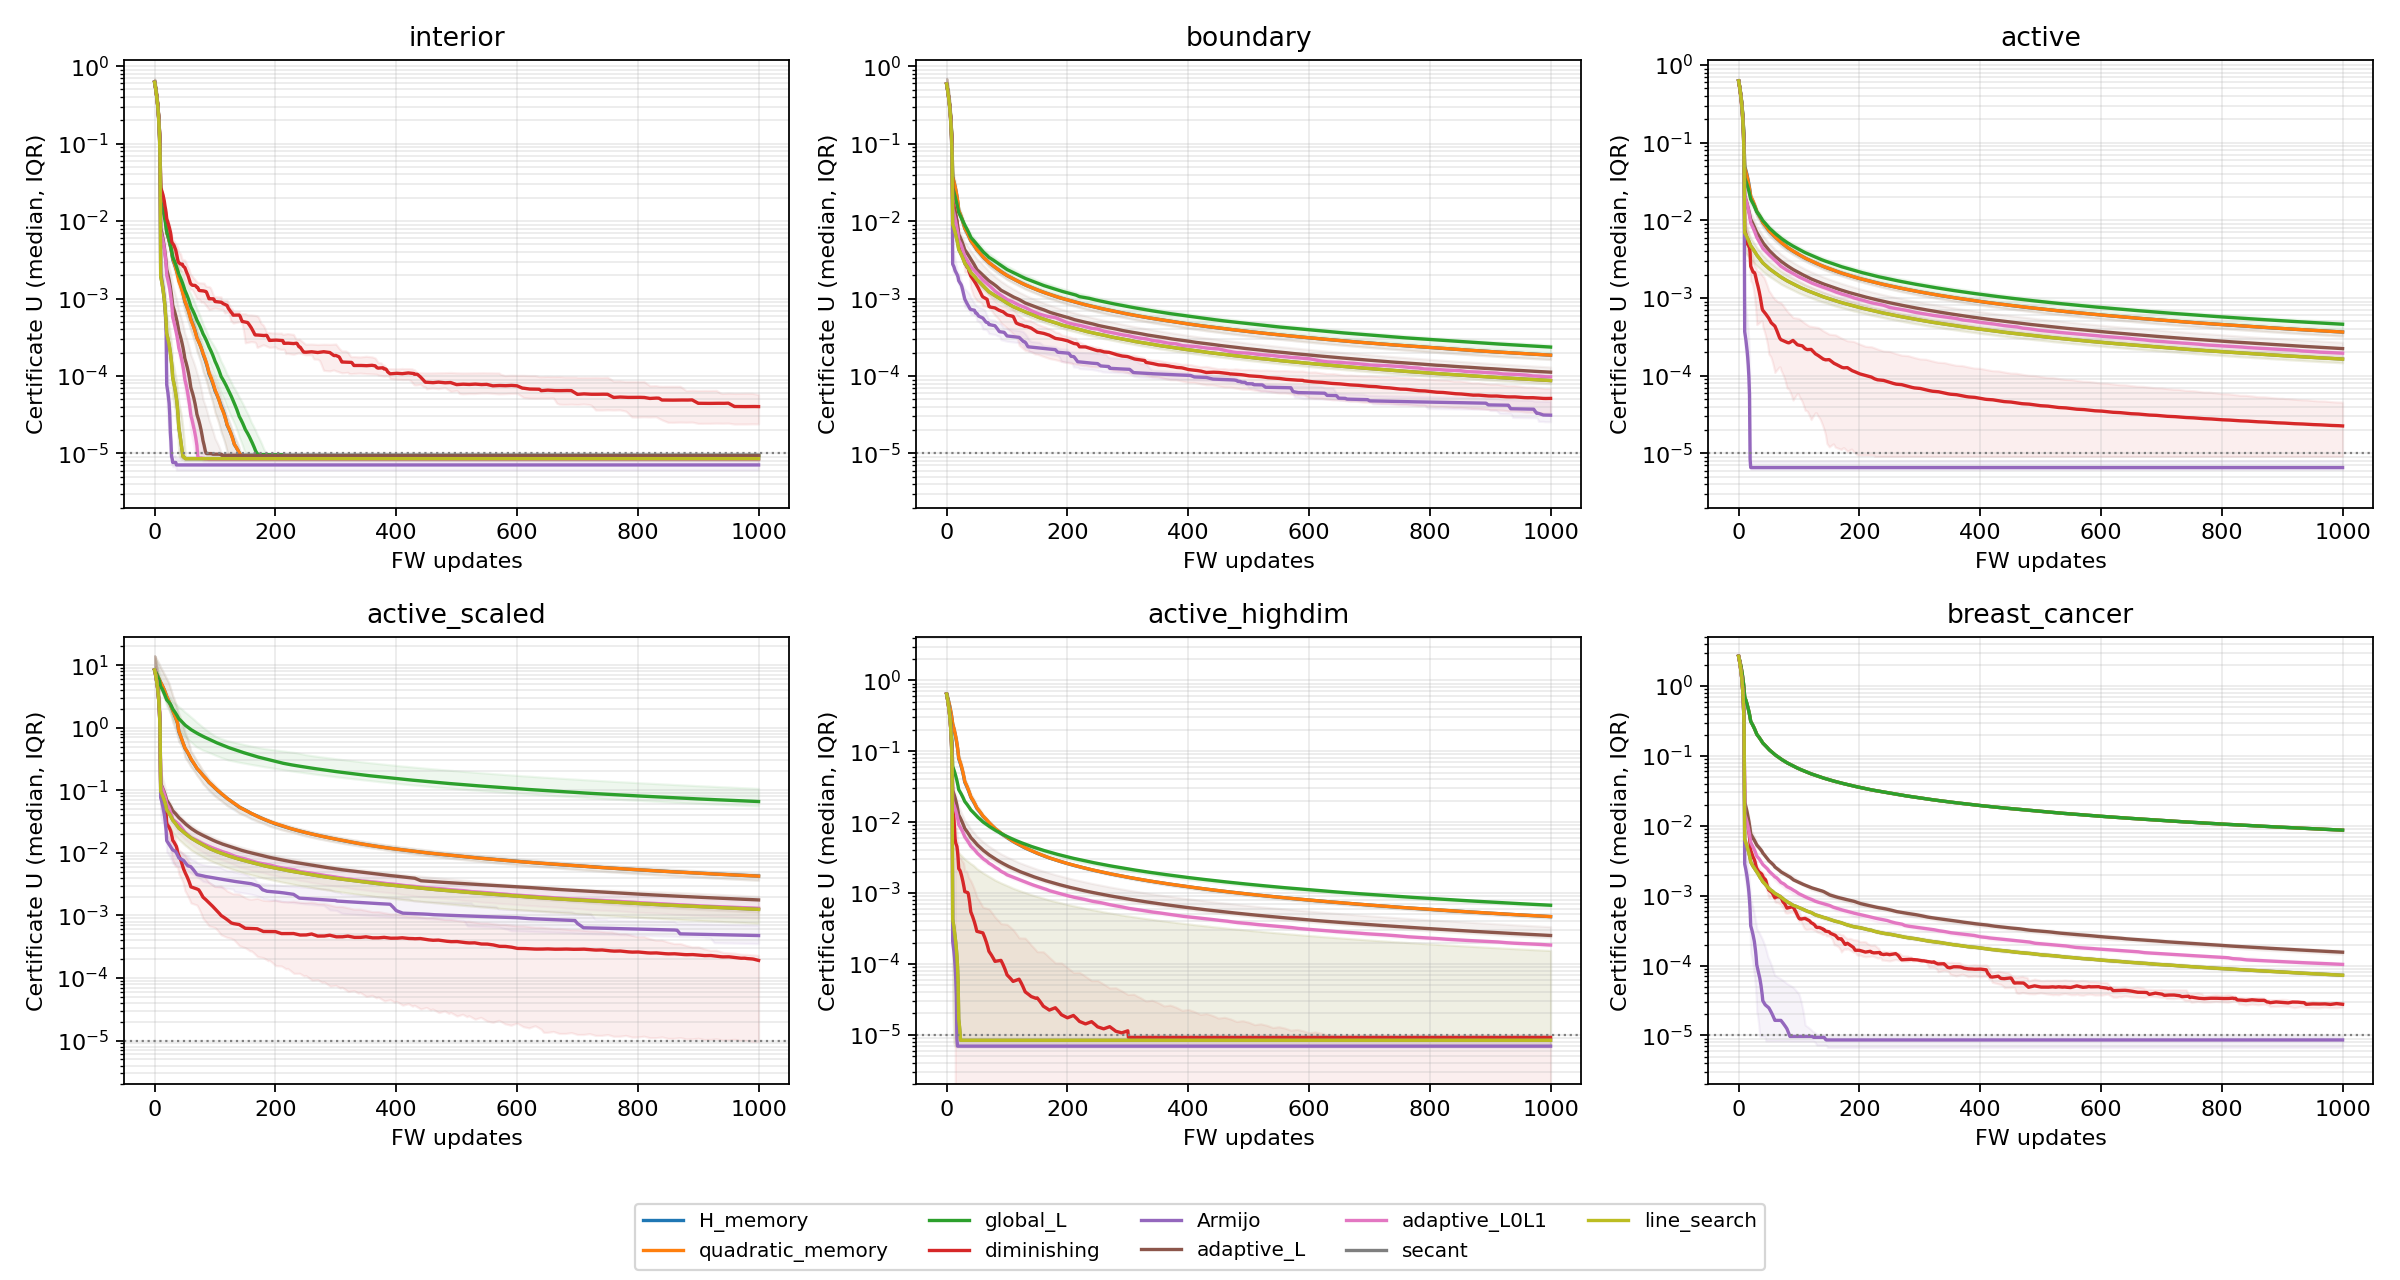
\includegraphics[width=\textwidth]{figures/certificates.png}
\caption{Median certificate and interquartile band across ten seeds.
Completed runs are carried forward at their final value. The figure uses
trace samples every ten updates plus the final point, linearly interpolated
for plotting only. The vertical display range is clipped below $2\cdot10^{-6}$;
actual values, including zero certificates, are retained in the CSV files.
The horizontal reference is the stopping tolerance $10^{-5}$.}
\label{fig:certificates}
\end{figure}

\subsection{Reproducibility and limitations}
From the PART3 directory, after installing its pinned requirements, run
\begin{verbatim}
python Work/benchmark.py --seeds 10 --max-iter 1000 --tolerance 1e-5
\end{verbatim}
The recorded environment uses Python 3.13.5, NumPy 2.5.2, SciPy 1.16.3,
Matplotlib 3.10.9, and scikit-learn 1.8.0, with BLAS/OpenMP thread
environment variables set to 1. The manifest records platform details,
parameters, reference intervals, and source SHA-256 hashes. Timings are
one run per instance, include logging, and exclude problem/reference
construction. They are exploratory; inter-seed variation does not replace
repeated timing on each instance. Function, gradient, and LMO costs are
reported separately, without assigning arbitrary relative weights.

Sixty-five automated tests compare the analytic minimizer with numerical
scalar minimization and check numerical derivatives, KKT conditions,
curvature bounds, local progress, certificates, oracle counts,
objective-shift invariance, independence from reference values, the
$H_1\to0$ limit, $H_0=0$, and deterministic error corrections.
Additional checks cover the adaptive envelope, exact telescoping identity,
total function-call bound, objective rescaling, unknown-curvature inputs,
and a positive-$H_1$ real-data problem, plus matching first steps in the
initialization ablation. Boundary tests cover both attainable quadratic
gap-envelope branches and the geometric theorem with $H_0=0$.
A separate exact-rational audit checks 8370 finite configurations,
including 57989 abstract curvature-state visits, phase-budget constants,
gap inversion and atom-removal counts. Its archived source and hashes
are replayed by the validator. The abstract state model dominates
possible curvature histories but does not assert realizability of
every state by an objective. Neither finite numerical checks nor this
rational audit establish a universal theorem or replace independent
proof review.

The companion focused article, \texttt{article.pdf}, strengthens the
pointwise gap envelope by a differential comparison with attaining
objectives. It also characterizes the zero-base optimal face and proves
finite exact termination of backtracking AFW in that regime, without
a separate geometric-growth assumption. This expanded report retains
the older valid quadratic comparisons to document the historical
experiments; their saved thresholds and outcomes are not recomputed.

\paragraph{Generative-tool disclosure.}
An OpenAI Codex assistant was used substantially for literature triage,
proof development, implementation, experiment analysis, manuscript
drafting and verification automation. Explicit derivations, archived
sources and executable checks are provided for scrutiny; this internal
process is not independent mathematical peer review. Responsibility for
submitted scientific claims rests with the named authors.

\subsection{Additional study: adaptation and real count data}
A separate recorded study repeats the controls with the adaptive method
and adds Poisson regression: 12 methods, seven scenarios, ten seeds, or
840 runs. These include reruns of previous controls, not 840 independent
new problem instances. The previous 660-run experiment and exact source
snapshots are retained. New results are in \texttt{Work/adaptive\_results/}.

For the official UCI Bike Sharing daily data~\cite{bike}, use the first
584 of 731 chronological observations. Training-only standardized
features are temperature, apparent temperature, humidity, windspeed,
working-day, holiday and year indicators, plus an intercept. The target
components \texttt{casual} and \texttt{registered} are excluded.
Let $t_i=y_i/\bar y$, where $y_i$ is the count and $\bar y$ its training
mean. On an $\ell_1$ ball of radius $R=1.5$, minimize
\[
 f(x)=\frac1m\sum_i\big[e^{a_i^\top x}-t_i a_i^\top x
                         +t_i\log t_i-t_i\big]+\frac\mu2\norm x^2,
 \quad \mu=0.01.
\]
This is a Poisson-deviance objective with offset $\log\bar y$, divided
by $\bar y$, plus the quadratic penalty. Seeds vary only the starting
signed vertex of this fixed training objective. No forecasting performance
claim or test-set evaluation is made.

For $H_1=\max_i\norm{a_i}^2$ and $C=m^{-1}\sum_i(t_i\log t_i-t_i)$,
$\norm{\nabla^2f}\le\mu+H_1m^{-1}\sum_i e^{a_i^\top x}$.
Also $f_Q^*\le f(0)=1+C$ and
$m^{-1}\sum_i t_i a_i^\top x\le Rm^{-1}\sum_i t_i\norm{a_i}_\infty$.
Thus~\eqref{eq:curvature} holds with the explicit, conservative constant
\[
 H_0=\mu+H_1\left(1+\frac Rm\sum_i t_i\norm{a_i}_\infty\right).
\]
Here $H_0\approx165.37$, $H_1\approx49.39$, while the guaranteed global
$L$ is approximately 8098.06. The independent SLSQP reference is polished
by Newton steps when interior and is accompanied by its FW-gap interval.
The reference is unavailable to every FW solver.

Table~\ref{tab:adaptive} gives selected results. On the real count
problem, certificate-scaled backtracking and the chosen adaptive-$L$
baseline each certify eight of ten starts. Their respective median
function-call counts are 860 and 1789, including capped runs.
Armijo certifies all ten starts, using 4399 median function calls and
310 updates. This is a promising comparison with one backtracking
configuration, not uniform superiority or a paired speedup for every start.
On the scaled active family, the new method certifies no run within
the cap. All 70 runs of the new method obey the total trial bound
in~\eqref{eq:trials}; this is a trajectory check, not a proof by experiment.
The real-data study covers only one dataset and radius with positive
$H_1$. The next subsection adds auto-conditioned FW~\cite{autoconditioned}.
\begin{table}[htbp]
\centering\small
\caption{Additional 840-run study: selected comparisons. Medians over ten seeds include capped runs; tolerance $10^{-5}$ and cap 1000 updates. On Bike Sharing, seeds vary the starting vertex of one fixed training objective.}
\label{tab:adaptive}
\begin{tabular}{lrrrrr}
\hline
Method & Successes & Updates & $U$ & $f$ calls & $\nabla f$ calls \\
\hline
\multicolumn{6}{l}{\textbf{interior}} \\
Hyperbolic, known $H_0,H_1$ & 10/10 & 136.5 & 9.48e-06 & 137.5 & 137.5 \\
Adaptive $L$ & 10/10 & 85.0 & 9.34e-06 & 168.5 & 86.0 \\
Certificate-scaled backtracking & 10/10 & 75.0 & 8.71e-06 & 168.0 & 76.0 \\
Armijo & 10/10 & 27.0 & 7.10e-06 & 220.0 & 28.0 \\
\hline
\multicolumn{6}{l}{\textbf{active\_scaled}} \\
Hyperbolic, known $H_0,H_1$ & 0/10 & 1000.0 & 4.25e-03 & 1001.0 & 1001.0 \\
Adaptive $L$ & 0/10 & 1000.0 & 1.77e-03 & 2002.0 & 1001.0 \\
Certificate-scaled backtracking & 0/10 & 1000.0 & 1.47e-03 & 2014.0 & 1001.0 \\
Armijo & 1/10 & 1000.0 & 4.78e-04 & 9758.0 & 1001.0 \\
\hline
\multicolumn{6}{l}{\textbf{bike\_poisson}} \\
Hyperbolic, known $H_0,H_1$ & 0/10 & 1000.0 & 1.04e-01 & 1001.0 & 1001.0 \\
Adaptive $L$ & 8/10 & 893.5 & 9.85e-06 & 1789.0 & 894.5 \\
Certificate-scaled backtracking & 8/10 & 419.0 & 9.41e-06 & 860.0 & 420.0 \\
Armijo & 10/10 & 310.0 & 9.93e-06 & 4399.0 & 311.0 \\
\hline
\end{tabular}
\end{table}


A 210-run ablation repeats the same seven families with three methods.
The new control uses the same initial curvature $U_0/D^2$ and the same
first trial as the proposed method, followed by ordinary halving of $L$
without current-certificate scaling. On Bike Sharing its median function
count is 1002.5, with six certified starts, versus 860 and eight for the
proposed method. The original baseline's count of 1789 therefore partly
reflects initialization. The median of the ten paired function-call ratios
is 0.953, with a descriptive 95\% percentile-bootstrap interval
$[0.535,2.303]$ (10000 resamples, seed 7103, capped runs included).
This wide interval includes 1; stable empirical superiority is not
established. On the interior family the corresponding median ratio is
1.050 with interval $[0.824,1.184]$. These are descriptive intervals
without multiple-comparison correction. The ablation reuses the main
instances and is not independent evidence from new datasets.
Theorem~\ref{thm:ordinary} now proves the same two-phase order for ordinary
backtracking, including an arbitrary positive initial estimate.

\subsection{Ordinary backtracking and an auto-conditioned comparator}
A separate 350-run extension uses the same seven families, ten seeds,
tolerance, and cap. It compares ordinary backtracking initialized at 1
or $U_0/D^2$, certificate scaling, Armijo, and AC-FW
\cite{autoconditioned}. Of these runs, 280 repeat existing deterministic
trajectories with additional logging; only the 70 AC-FW runs add a new
method on these same instances. They are not new independent datasets.

AC-FW is our independent implementation of Algorithms 1 and 2 in
\cite{autoconditioned}, using its equation (6) with a fixed $\delta=1$:
\[
 r_t=1-\frac{1}{(t+1)\log^2(t+3)}.
\]
We do not claim to reproduce the authors' numerical configuration.
Its compulsory move from $x_{-1}$ to an LMO vertex $x_0$, both function
and gradient evaluations, and the initial LMO are charged. Available
linear lower bounds from both points enter the certificate history.
After initialization, each outer iteration makes one function trial;
strict decrease accepts the point, and rejection keeps the old point
and cached gradient. Rejections consume the iteration cap. Consequently
$N_f=N+2$, $N_{\rm LMO}=N+2$, and $N_g=2+N_{\rm accepted}$, including the
final certificate check. The initial move changes the starting trajectory;
its effect is included in the algorithm comparison, not isolated in an
initialization ablation. Our cosh and Poisson losses are not globally
gradient-Lipschitz on $\R^d$, unlike the assumption in the cited paper;
their use here is an empirical comparison on the compact feasible set,
not a claim that its global theorem applies verbatim.

Table~\ref{tab:backtracking} shows strong competing results. On the active
family AC-FW certifies all ten runs, with medians 18.5 function and gradient
calls; certificate scaling certifies one run within the cap. On the scaled
active family neither adaptive variant nor AC-FW certifies any run, and
AC-FW's median certificate is worse. On Bike Sharing AC-FW uses 639 median
function calls and certifies seven starts, versus 860 calls and eight
starts for certificate scaling; its median gradient count is higher
(639 versus 420). Capped runs remain in every median, so these figures
must be read together with successes and both oracle budgets. Only five
outer trials are rejected across the 70 AC-FW runs. This study gives no
uniform practical ranking or evidence that the normalization is necessary.

We replay all 140 ordinary-backtracking runs from their archived source
and check every accepted curvature, decrease, phase classification,
lag budget, telescoping trial identity, and trial bound. The replay
matches recorded objectives, certificates, and all three oracle counts
exactly. All these runs have zero lag steps relative to the conservative
analytic phase caps; they do not test sharpness of the lag bound or the
large worst-case iteration constants. A separate affine example tests
more than twenty lag steps and the exact formula in
Proposition~\ref{prop:initialization}. Five hundred abstract trajectories
stress the potential argument with abrupt phase jumps and varying
initial scales. These checks support implementation consistency, not
independent mathematical validation or a priority claim.

\begin{table}[htbp]
\centering\small
\caption{350-run extension, selected families. Medians include capped runs. The cap is 1000 outer iterations, including AC-FW rejections; the compulsory AC-FW initialization is included in all oracle costs. Success means $U\le10^{-5}$.}
\label{tab:backtracking}
\begin{tabular}{lrrrrr}
\hline
Method & Successes & Outer iterations & $U$ & $f$ calls & $\nabla f$ calls \\
\hline
\multicolumn{6}{l}{\textbf{active}} \\
Ordinary, $M=U_0/D^2$ & 1/10 & 1000.0 & 2.43e-04 & 2002.0 & 1001.0 \\
Ordinary, $M=1$ & 0/10 & 1000.0 & 2.23e-04 & 1998.5 & 1001.0 \\
Certificate scaling & 1/10 & 1000.0 & 1.99e-04 & 2014.0 & 1001.0 \\
AC-FW, $\delta=1$ & 10/10 & 16.5 & 7.93e-06 & 18.5 & 18.5 \\
Armijo & 10/10 & 19.0 & 6.55e-06 & 141.0 & 20.0 \\
\hline
\multicolumn{6}{l}{\textbf{active\_scaled}} \\
Ordinary, $M=U_0/D^2$ & 0/10 & 1000.0 & 1.87e-03 & 2002.0 & 1001.0 \\
Ordinary, $M=1$ & 0/10 & 1000.0 & 1.77e-03 & 2002.0 & 1001.0 \\
Certificate scaling & 0/10 & 1000.0 & 1.47e-03 & 2014.0 & 1001.0 \\
AC-FW, $\delta=1$ & 0/10 & 1000.0 & 2.67e-03 & 1002.0 & 1002.0 \\
Armijo & 1/10 & 1000.0 & 4.78e-04 & 9758.0 & 1001.0 \\
\hline
\multicolumn{6}{l}{\textbf{bike\_poisson}} \\
Ordinary, $M=U_0/D^2$ & 6/10 & 500.0 & 9.87e-06 & 1002.5 & 501.0 \\
Ordinary, $M=1$ & 8/10 & 893.5 & 9.85e-06 & 1789.0 & 894.5 \\
Certificate scaling & 8/10 & 419.0 & 9.41e-06 & 860.0 & 420.0 \\
AC-FW, $\delta=1$ & 7/10 & 637.0 & 9.53e-06 & 639.0 & 639.0 \\
Armijo & 10/10 & 310.0 & 9.93e-06 & 4399.0 & 311.0 \\
\hline
\end{tabular}
\end{table}


\subsection{Separating vertex initialization from the update rule}
The preceding AC-FW comparison changes both initialization and the
subsequent rule. We therefore run a controlled $2\times2$ study on the
same 70 instances: the original point or the compulsory LMO vertex,
combined with AC updates or ordinary backtracking (BT). All four cells
pay for two function values, two gradients, and two LMOs at the two
preprocessing points. They retain both scalar lower bounds and the same
secant curvature. BT's stored initial estimate is twice the AC estimate,
so its first halving gives exactly the same first trial. Afterwards BT
halves and doubles its estimate, while AC uses the fixed damping above.
AC/vertex is the native comparator; the other three cells are controls,
not the published AC-FW algorithm. No curvature or reference quantities
are supplied to their step rules.

There are 280 runs with the previous outer cap and tolerance. All 70
AC/vertex runs match the earlier native comparator's objective,
certificate, and oracle counts exactly; no new independent instances
are added. Table~\ref{tab:factorial} uses separate budgets for function
and gradient calls. Each value is the last fully available certificate
before that oracle budget, reconstructed from the complete trace before
sampling. It is not an interpolation between saved trace rows. Other
oracle types are unrestricted. All nonterminal runs can reach 1000
function calls before hitting the outer cap, so this primary budget
comparison is not censored by that cap.

On the active family, moving to the LMO vertex changes the number of
certified runs at 1000 function calls from 1 to 10 for AC and from 0 to
10 for BT. Thus the earlier 10/10 versus 0--1/10 comparison did not
isolate the subsequent curvature update. The median paired certificate
ratio BT/AC from the vertex is 1.049, with descriptive percentile-bootstrap
interval $[0.935,1.257]$. Vertex/original ratios are 0.0351 for AC and
0.0150 for BT. These describe the ten matched instances at a fixed
budget, not speedup factors or a population-level ranking; completed
runs stop near the tolerance. All 84 comparisons, including other
oracle budgets and families, are recorded with 10000 bootstrap resamples
and seed 20261015, without a multiple-comparison correction.

On Bike Sharing at 1000 function calls, AC certifies 6/10 starts from the
original point and 7/10 from the vertex; BT certifies 2/10 and 5/10.
At 1000 gradients BT/original certifies 6/10, like AC/original. The oracle
unit changes the comparison. The scaled active family remains unsolved
by all four cells within the reported budgets. Figure~\ref{fig:initialization}
shows the function-budget profiles.

\begin{table}[htbp]
\centering\small
\caption{Controlled starting-point/update-rule ablation. Each cell has the same preprocessing cost and first trial curvature. Successes and median certificates at separate budgets of 1000 function or gradient calls, over ten seeds. Other oracle types are unrestricted; the outer cap remains 1000.}
\label{tab:factorial}
\begin{tabular}{llrrrr}
\hline
 & & \multicolumn{2}{c}{1000 function calls} & \multicolumn{2}{c}{1000 gradient calls} \\
Rule & Start & Successes & Median $U$ & Successes & Median $U$ \\
\hline
\multicolumn{6}{l}{\textbf{active}} \\
AC & original & 1/10 & 2.06e-04 & 1/10 & 2.06e-04 \\
AC & vertex & 10/10 & 7.93e-06 & 10/10 & 7.93e-06 \\
BT & original & 0/10 & 5.18e-04 & 0/10 & 2.61e-04 \\
BT & vertex & 10/10 & 8.44e-06 & 10/10 & 8.44e-06 \\
\hline
\multicolumn{6}{l}{\textbf{active\_scaled}} \\
AC & original & 0/10 & 2.00e-03 & 0/10 & 2.00e-03 \\
AC & vertex & 0/10 & 2.68e-03 & 0/10 & 2.68e-03 \\
BT & original & 0/10 & 3.72e-03 & 0/10 & 1.86e-03 \\
BT & vertex & 0/10 & 3.60e-03 & 0/10 & 1.84e-03 \\
\hline
\multicolumn{6}{l}{\textbf{bike\_poisson}} \\
AC & original & 6/10 & 9.72e-06 & 6/10 & 9.72e-06 \\
AC & vertex & 7/10 & 9.53e-06 & 7/10 & 9.53e-06 \\
BT & original & 2/10 & 6.72e-05 & 6/10 & 9.94e-06 \\
BT & vertex & 5/10 & 2.20e-05 & 5/10 & 1.11e-05 \\
\hline
\end{tabular}
\end{table}


\paragraph{A geometric explanation on the planted instances.}
Let $w=\operatorname{sign}(x^*)$, zero off its support, and
$\sigma(x)=R-w^\top x\ge0$. The optimal face is
$F=\{x\in Q:\sigma(x)=0\}$. Every FW update satisfies exactly
\[
 \sigma(x+\alpha(s-x))=(1-\alpha)\sigma(x)+\alpha\sigma(s).
\]
If selected vertices lie in $F$ and all steps are strictly below 1,
a point outside $F$ retains positive slack at every finite iteration.
A full initial move to a vertex in $F$ removes this slack immediately.
For the planted normal $v$, $|v_i|\le0.6$ off the support, so
\[
 f(x)\ge\lambda(R-v^\top x)\ge0.4\lambda\sigma(x).
\]
The last inequality uses $\|x_{\rm off}\|_1\le\sigma(x)$.
This is an application of the familiar face geometry of vanilla
FW~\cite{braun}, not a new acceleration mechanism.

Post-run diagnostics replay all 120 controls in the three active families,
using the planted support only after solving. The slack identity and
lower bound hold throughout. On the active family the initial LMO vertex
lies in $F$ for all ten seeds, and both vertex-start cells stay in $F$.
BT/original takes no full step and retains positive final slack in all
ten runs; AC/original takes one full step in its sole successful run.
At the outer cap, BT/original's smallest final slack among these ten
runs is about $9.98\cdot10^{-4}$. Since $\lambda=0.15$, the lower
bound above already exceeds the target $10^{-5}$ in every run;
failure here is not merely a loose stopping certificate.
In the high-dimensional family the initial vertex is in $F$ for eight
seeds, and the corresponding vertex-start runs stay there. In the scaled
family only one initial vertex is in $F$, and no vertex-start run remains
in $F$ throughout. This explains the observed initialization sensitivity
on these constructed examples without a claim for general applications.

\begin{figure}[htbp]
\centering
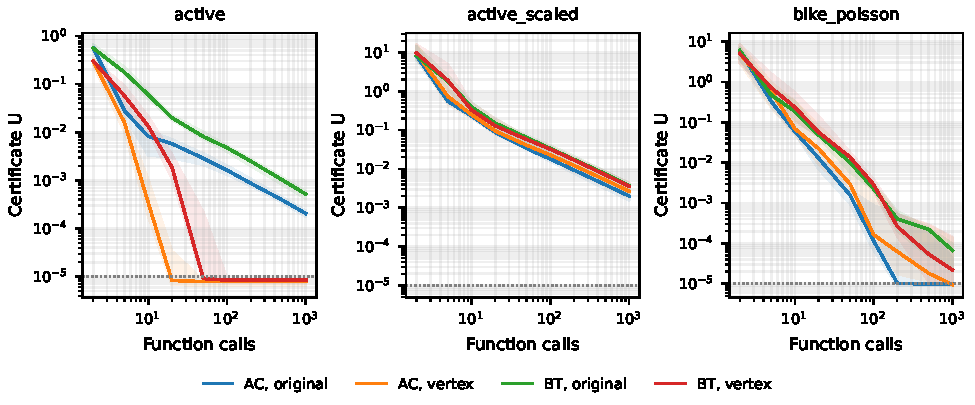
\includegraphics[width=\textwidth]{figures/initialization_effect.pdf}
\caption{Controlled ablation: median certificate and interquartile band
at the displayed function-call budgets. Every prefix includes common
preprocessing. Runs stop at $U\le10^{-5}$ or 1000 outer trials; completed
certificates are carried forward. The displayed function budgets are
reached before the outer cap in nonterminal runs. Lines between displayed
budgets are for visualization; the CSV contains the actual prefix values.}
\label{fig:initialization}
\end{figure}

\subsection{Away-step comparison from the original point}
The initialization study motivates a direction-level control. We compare
FW and AFW, each with ordinary backtracking (BT) or the explicit
known-$H$ quadratic step (Q), on the same 70 instances. All four methods
start at the original vertex, without a compulsory initial move.
BT starts at estimate 1, halves before each search, and doubles on
rejection. Q uses $H_0+H_1U_k$. AFW chooses the stronger FW/away
direction and respects its active-weight cap. The certificate uses the
full FW gap even on away steps. This is an implementation of established
algorithms, not a newly proposed AFW direction rule.

The 280 runs include 140 exact repeats of the earlier two FW baselines,
verified against their saved objectives, certificates and oracle counts.
The 140 AFW runs add method comparisons on existing instances, rather
than new independent tasks. Table~\ref{tab:away} distinguishes the
outer cap of 1000 updates from a fixed budget of 1000 function calls.
The budget values use complete trajectory prefixes. Function, gradient
and full-LMO calls are reported separately; each method uses $N+1$
gradients and full LMOs. AFW additionally scans its active set once per
update, and records the number of atom scores. Maintaining and
reconstructing active weights also costs work, so oracle counts alone
do not establish a wall-clock advantage.

AFW-BT reaches $U\le10^{-5}$ in all 70 runs within the outer cap.
On the scaled active family, it certifies 10/10 instances, using medians
56.5 function calls and 28.5 gradients. FW-BT certifies none within the
cap. On the breast-cancer control, AFW-BT certifies 10/10 with 103.5
median function calls, versus 0/10 for FW-BT. On Bike Sharing AFW-BT
certifies 10/10 by the end, but only 6/10 at 1000 function calls; the
corresponding FW-BT count at that budget is 1/10. End-of-run medians
include capped runs and must be read with these successes.

AFW-Q still certifies no run of either real regression within 1000
updates. Thus active-set correction alone does not make a conservative
analytic step efficient on these data. On the interior family, the
FW/AFW differences are modest. Figure~\ref{fig:away} shows the fixed
function-budget profiles; it does not establish a ranking over all
projection-free methods or untested instances.

Every step of the 70 AFW-BT trajectories is checked before trace
sampling: accepted-curvature envelope, dyadic trial identity, local
decrease, phase lag budget, drop count, and total function-call bound.
The certificate bridge is checked using the independent reference
interval and the analytically valid ridge lower bound on strong
convexity. No positive weights are pruned heuristically in these runs,
and no unexpected numerical atom deletions occur. A separate interval
test, where the geometric width is explicit, checks
\eqref{eq:awaygeometry} and the strongly convex phase bound. A geometric
constant is not fitted to the benchmark trajectories, and these finite
checks do not independently validate the general theorem.

\begin{table}[htbp]
\centering\small
\caption{FW versus AFW from the same original point, ten matched seeds. Final medians include capped runs; the cap is 1000 updates. The last columns use a separate budget of 1000 function calls.}
\label{tab:away}
\begin{tabular}{lrrrrr}
\hline
Method & Final successes & $f$ calls & $\nabla f$ calls & Successes at 1000 $f$ & Median $U$ \\
\hline
\multicolumn{6}{l}{\textbf{active\_scaled}} \\
FW\_BT & 0/10 & 2002.0 & 1001.0 & 0/10 & 3.28e-03 \\
AFW\_BT & 10/10 & 56.5 & 28.5 & 10/10 & 7.94e-06 \\
FW\_Q & 0/10 & 1001.0 & 1001.0 & 0/10 & 4.26e-03 \\
AFW\_Q & 10/10 & 160.5 & 160.5 & 10/10 & 8.67e-06 \\
\hline
\multicolumn{6}{l}{\textbf{breast\_cancer}} \\
FW\_BT & 0/10 & 1997.0 & 1001.0 & 0/10 & 3.11e-04 \\
AFW\_BT & 10/10 & 103.5 & 53.5 & 10/10 & 9.52e-06 \\
FW\_Q & 0/10 & 1001.0 & 1001.0 & 0/10 & 8.67e-03 \\
AFW\_Q & 0/10 & 1001.0 & 1001.0 & 0/10 & 1.24e-03 \\
\hline
\multicolumn{6}{l}{\textbf{bike\_poisson}} \\
FW\_BT & 8/10 & 1789.0 & 894.5 & 1/10 & 3.01e-05 \\
AFW\_BT & 10/10 & 877.5 & 439.0 & 6/10 & 9.88e-06 \\
FW\_Q & 0/10 & 1001.0 & 1001.0 & 0/10 & 1.04e-01 \\
AFW\_Q & 0/10 & 1001.0 & 1001.0 & 0/10 & 1.00e-01 \\
\hline
\end{tabular}
\end{table}

\begin{figure}[htbp]
\centering
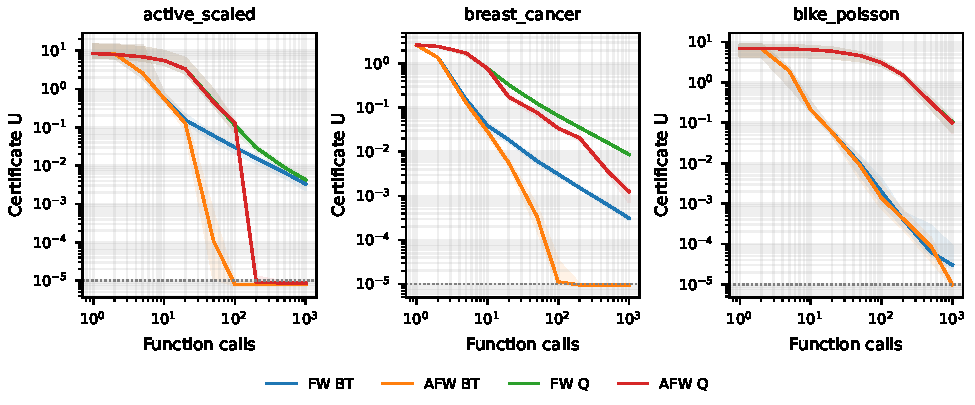
\includegraphics[width=\textwidth]{figures/away_comparison.pdf}
\caption{FW versus AFW from a common original start. Median certificate
and interquartile band at displayed function-call budgets. Completed
runs are carried forward. Every nonterminal run reaches the displayed
budgets before the outer cap. Lines between budgets are for display;
the CSV stores actual available certificates. Q methods receive analytic
curvature constants; BT methods do not. Active-set work is additional.}
\label{fig:away}
\end{figure}

\subsection{Radius and objective-unit controls}
\label{sec:robustness}
The final control varies the radius while keeping each real-data objective
fixed. The logistic radii are $1,2,4$ and the Poisson radii are
$0.75,1.5,3$. Each radius has a newly computed constrained reference
interval; the Poisson curvature bounds are recomputed on its new domain.
Five matched seeds and objective scales $a\in\{10^{-3},1,10^3\}$ give
360 runs of four methods: FW/AFW with either $M=1$ or $M=U_0/D^2$.
The target for $af$ is $a10^{-5}$, so all conditions use the same
accuracy in original units. No reference or curvature constants are
solver inputs, and certificate initialization reuses the first paid
function, gradient, and LMO evaluations. The 30 unscaled default-radius
baselines agree exactly with their earlier records.

\begin{proposition}[Objective units in halving backtracking]
\label{prop:units}
In exact arithmetic, replace $f$ by $\widetilde f=af+b$, $a>0$, and
$\varepsilon$ by $a\varepsilon$. For FW or AFW, scale $M$ by $a$ and
use identical scale-invariant tie breaking. Then all iterates, accepted
steps, trial counts, and stopping indices are unchanged. In particular,
$M=U_0/D^2$ makes this scaling automatic. Keeping $M$ fixed instead
corresponds to initialization $M/a$ on the original objective.
\end{proposition}
\begin{proof}
Every tangent lower bound transforms as $\widetilde\ell=a\ell+b$,
and $\widetilde G=aG$, $\widetilde U=aU$. Positive scaling preserves
LMO and away-atom comparisons. Inductively $\widetilde L=aL$, so the
ratio of directional gap to $L\norm d^2$, the feasible cap, and the
quadratic acceptance comparison are unchanged. Halving and doubling
commute with positive scaling. The stopping test scales identically.
\end{proof}
This elementary property is an initialization control, not a new
convergence result. The curvature parameters transform as
$\widetilde H_0=aH_0$, $\widetilde H_1=H_1$; strong convexity scales
as $\widetilde\mu=a\mu$.

Both AFW initializations certify all 90 radius/seed/scale conditions
within 1000 updates. FW certifies 30/90 with fixed $M$ and 33/90 with
certificate initialization. These counts include repeated scalings of
the same problems and are not independent replications. At scale one,
the certificate-initialized AFW function-call median increases from
73 to 388 as the logistic radius goes from 1 to 4; all five seeds
still finish. At Poisson radius 3, that median is 1292 and only 1/5
seeds finish within 1000 function calls. Thus success within the update
cap is distinct from success at a fixed function budget.

Objective units can affect more than the final call count. For logistic
radius 1, FW with fixed $M=1$ certifies 0/5 at $a=10^{-3}$ but 5/5 at
$a=1$ and $10^3$. For both certificate-initialized methods, all 60
matched scale comparisons preserve final function/gradient/LMO counts
and stopping outcomes. The maximum relative change in $U/a$ across
the recorded oracle-budget prefixes is below $3.2\cdot10^{-11}$,
using denominator $\max\{10^{-5},U_{a=1}\}$. This compares recorded
certificates and counters, not bitwise equality of complete iterates;
finite precision can change branch decisions in general.

All logistic references are on the constraint boundary. The Poisson
reference has $\ell_1$ norm approximately 0.692 and is interior at
all three radii. Thus this control does not test an active Poisson
constraint. No new dataset or predictive-performance claim is added.
Changing the radius changes both the domain and its original starting
vertex. Certificate initialization is not uniformly faster than the
fixed initialization. Additional AFW active-set work remains separately
counted, and no wall-clock ranking follows.

\begin{table}[htbp]
\centering\small
\caption{Radius controls at objective scale $a=1$, five matched seeds. Each entry gives final successes (out of five); median function calls. Capped failures are included. The cap is 1000 updates, not 1000 function calls. Subscript $1$: $M=1$; subscript $U$: $M=U_0/D^2$.}
\label{tab:robustness}
\begin{tabular}{lrrrr}
\hline
Radius & FW$_1$ & FW$_U$ & AFW$_1$ & AFW$_U$ \\
\hline
\multicolumn{5}{l}{\textbf{breast\_cancer}} \\
$R=1$ & 5; 205 & 5; 161 & 5; 83 & 5; 73 \\
$R=2$ & 0; 1997 & 0; 1999 & 5; 105 & 5; 101 \\
$R=4$ & 0; 1998 & 0; 2000 & 5; 342 & 5; 388 \\
\hline
\multicolumn{5}{l}{\textbf{bike\_poisson}} \\
$R=0.75$ & 0; 2002 & 0; 2003 & 5; 829 & 5; 906 \\
$R=1.5$ & 4; 1804 & 4; 423 & 5; 791 & 5; 635 \\
$R=3$ & 3; 1920 & 2; 1999 & 5; 1085 & 5; 1292 \\
\hline
\end{tabular}
\end{table}

\begin{figure}[htbp]
\centering
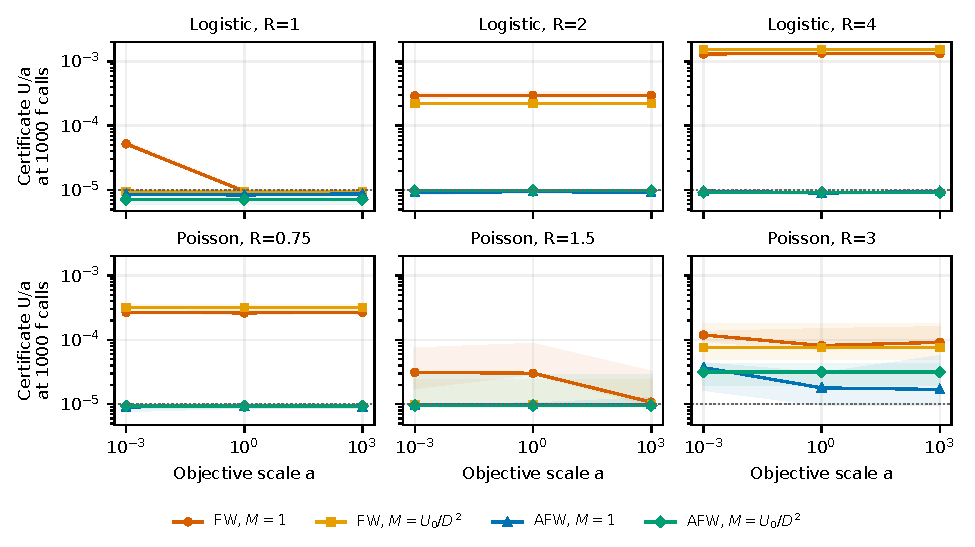
\includegraphics[width=\textwidth]{figures/radius_and_units.pdf}
\caption{Radius and objective-unit controls. Median and interquartile
band of the certificate in original units, $U/a$, after at most 1000
function calls, five matched seeds. The tolerance is $10^{-5}$ in these
units. Completed runs are carried forward; nonterminal runs reach the
displayed budget before the update cap. Lines only connect the three
tested scales. Scaled versions of a problem are paired controls.}
\label{fig:robustness}
\end{figure}

\subsection{A Poisson constraint-activity transition}
\label{sec:transition}
The preceding Poisson radii all leave the reference interior. We now fix
that objective and vary $R/R_*$ over the seven predefined values
$0.5,0.9,0.99,1,1.01,1.1,2$. Here $R_*\simeq0.691643204469$ is the
$\ell_1$ norm of an independently computed stationary point. Ridge
strong convexity gives the residual estimate
\[
 \bigl|\norm{x_{\rm ref}}_1-\norm{x^*_{\rm unc}}_1\bigr|
 \le \sqrt d\norm{\nabla f(x_{\rm ref})}/\mu.
\]
The numerical right-hand side is about $4.1\cdot10^{-15}$.
These are floating-point residual calculations, not interval arithmetic.
The radius equal to the numerical estimate is marked transitional;
the other regimes are separated from the estimate by much larger margins.
The three smaller ratios give active references with positive estimated
KKT multipliers; the three larger ones give interior references.
References and activity information are unavailable to the algorithms.

There are 280 raw trajectories of the same four FW/AFW backtracking
variants, to $U\le10^{-7}$ or 2000 updates. Their nested prefixes record
first attainment of $10^{-3},10^{-5},10^{-7}$ and separate oracle
budgets. Ten seed labels produce only seven distinct initial vertices:
seeds 6, 7, and 8 repeat seeds 1, 0, and 2, respectively. All stored
non-timing records for those 84 repeated trajectories agree exactly.
The primary table and figure retain one representative per vertex,
giving 196 distinct method/radius/start trajectories. These share
one dataset and one objective; they are not independent dataset
replications. Earlier seed-weighted tables retain their original
protocol, and should also be read with this multiplicity in mind.

Both AFW variants attain $10^{-7}$ on all 49 distinct radius/start
conditions. FW with $M=1$ attains it on 4/49, and FW with $M=U_0/D^2$
on 5/49. In the transitional region neither FW variant reaches
$10^{-7}$ within the cap. At $R/R_*=2$, certificate initialization
allows FW to finish on 4/7 starts, with median final cost 870 function
calls including capped failures; AFW finishes on 7/7, with median 1946
for that initialization. Capped medians alone therefore do not define
a ranking. The certificate initialization is also slower than $M=1$
for AFW at several radii. Active constraints, starting vertices,
solution support, and conditioning all change with radius; this is
not an isolation of one geometric constant or a universal ranking.

Every source of all 280 raw trajectories is checked against the local
gap envelope in Lemma~\ref{lem:awaybridge}, using
$\delta\le f(x)-f^*_{\rm ref,lower}$. The new threshold reduces the
analysis phase count before rounding by about 15--34 compared with
the previous distance-based threshold on these cases. It changes the
proof, not the algorithm or measured cost. No geometric constant
$\kappa$ is fitted. Estimated reference supports use threshold
$10^{-7}$; their final face-slack diagnostics do not certify exact
finite face identification. Active-set work is additional to the
function, gradient, and full-LMO counts.

\begin{table}[htbp]
\centering\small
\caption{Poisson transition sweep, 7 distinct starting vertices per radius. Entries are successes at $10^{-7}$ (out of 7); median final function calls, including failures capped at 2000 updates. Subscripts give $M=1$ or $M=U_0/D^2$.}
\label{tab:transition}
\begin{tabular}{lrrrr}
\hline
$R/R_*$ & FW$_1$ & FW$_U$ & AFW$_1$ & AFW$_U$ \\
\hline
0.5 & 2; 4002 & 1; 4003 & 7; 1399 & 7; 1043 \\
0.9 & 0; 4002 & 0; 4003 & 7; 1036 & 7; 1331 \\
0.99 & 0; 4001 & 0; 4003 & 7; 1150 & 7; 1585 \\
1 & 0; 4002 & 0; 4003 & 7; 1387 & 7; 1842 \\
1.01 & 0; 4001 & 0; 4003 & 7; 1396 & 7; 1862 \\
1.1 & 0; 4002 & 0; 4003 & 7; 1360 & 7; 1730 \\
2 & 2; 4001 & 4; 870 & 7; 1697 & 7; 1946 \\
\hline
\end{tabular}
\end{table}

\begin{figure}[htbp]
\centering
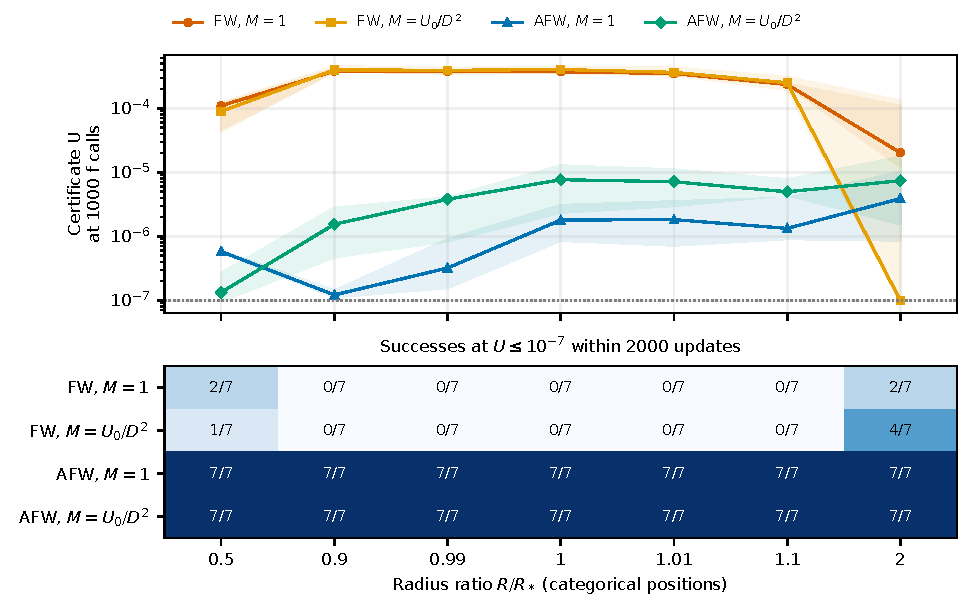
\includegraphics[width=\textwidth]{figures/constraint_transition.pdf}
\caption{Poisson activity sweep with equal weights on seven distinct
starts per radius. Top: median and interquartile certificate at 1000
function calls; completed runs are carried forward, and nonterminal
runs reach this budget. Bottom: successes at $10^{-7}$ within 2000
updates. Radius ratios occupy categorical positions, so their spacing
does not represent Euclidean distance. This is one dataset.}
\label{fig:transition}
\end{figure}

\subsection{Two additional count datasets and a limit of the certificate}
\label{sec:multidata}
We add Seoul Bike Sharing Demand~\cite{seoul} and Metro Interstate
Traffic Volume~\cite{metro}. The official files, their SHA-256 values,
and CC BY 4.0 attribution are retained. A stable chronological sort
followed by the first 80\% of rows gives 7008 Seoul observations with
15 model coordinates and 38563 Metro observations with 12 coordinates.
Repeated source timestamps retain their original weights.
Fixed feature choices include weather, cyclic time features, holiday,
and Seoul's functioning indicator; other textual categories are omitted.
Each non-intercept feature becomes
$\tanh((v-\bar v_{\rm train})/s_{\rm train})$ using training statistics
only. This bounded-feature protocol differs from the earlier Bike
Sharing standardization. Predictive accuracy is not evaluated.

The normalized Poisson deviance and ridge coefficient $\mu=0.01$ are
as before; the intercept is also constrained and regularized. Since
$\norm{a_i}_\infty=1$ and the normalized response $t_i$ has mean one,
valid radius-$R$ bounds are
\[
 H_1=\max_i\norm{a_i}^2,\quad H_0=\mu+H_1(1+R),\quad
 L_Q=\mu+e^R\lambda_{\max}(A^\top A/m).
\]
The Hessian norm is at most
$\mu+H_1\operatorname{mean}(e^{a_i^\top x})$; comparing $f_Q^*$ with
$f(0)$ yields $\operatorname{mean}(e^{a_i^\top x})\le\delta+1+R$.
Thus the condition holds relative to the constrained minimum. These
are upper bounds, not minimal curvature parameters, and positive
$H_1$ is not claimed necessary on a compact domain.

Offline damped Newton solves estimate $R_*:=\norm{x^*_{\rm unc}}_1$.
The values are approximately 4.575821 (Seoul) and 1.431745 (Metro). We compare
$R/R_*=1/2$ and 2, with independently recomputed active and interior
reference intervals of width below $4.3\cdot10^{-8}$. All 30 Seoul or
24 Metro signed coordinate vertices are used once per radius. Six
existing variants give 648 trajectories: the four BT variants and
FW/AFW known-$H$ short steps. The cap is 1000 updates, the tolerance
$10^{-5}$. References, activity and $R_*$ are offline information, not
solver inputs. Starts and radii within each dataset share data.

Both AFW-BT variants finish all 30 active Seoul and all 24 active Metro
starts. Their function-call medians are 424 versus 399 and 99 versus
80.5 for $M=1$ versus $M=U_0/D^2$, respectively. The interior controls
are unfavorable: neither AFW-BT variant finishes any Seoul start,
and only 6/24 and 7/24 finish on Metro. AFW-Q finishes all active Metro
starts with median 423 function/gradient calls, but no start in the
other three cases. These results limit any practical-success claim
based on the earlier Bike Sharing controls. All full trajectories
pass descent, feasibility, trial-count, active-removal, and local-gap
checks before sampling.

The independent reference interval distinguishes primal error from
the online certificate. At the interior Metro radius, every BT run
has post-run upper error
$e_{\rm ref}=\max\{0,f(x)-f^*_{\rm ref,lower}\}\le10^{-5}$.
Yet FW has no online $U$ successes and AFW has only 6 and 7. On
interior Seoul, 12/30 and 18/30 AFW runs have $e_{\rm ref}\le10^{-5}$,
although neither variant stops. Noncompletion can therefore reflect
both remaining primal error and a conservative observable certificate.
References do not replace actual stopping outcomes. Tighter dual
certificates merit investigation with their extra linear oracles
properly counted. Active-set work is additional, and no wall-clock
ranking follows from these counts.

\begin{table}[htbp]
\centering\small
\caption{Additional count datasets, every signed coordinate vertex. Entries: successes; median final function calls including failures capped at 1000 updates. Seoul has 30 starts per radius, Metro 24. $F/A$: FW/AFW; subscripts $1,U$: initial $M=1,U_0/D^2$; $Q$: known-$H$ short step.}
\label{tab:multidata}
\begin{tabular}{lrrrrrr}
\hline
$R/R_*$ & $F_1$ & $F_U$ & $A_1$ & $A_U$ & $F_Q$ & $A_Q$ \\
\hline
\multicolumn{7}{l}{\textbf{seoul}} \\
0.5 & 1; 2001 & 1; 2003 & 30; 424 & 30; 399 & 0; 1001 & 0; 1001 \\
2 & 0; 2001 & 0; 1996 & 0; 2001 & 0; 1995.5 & 0; 1001 & 0; 1001 \\
\hline
\multicolumn{7}{l}{\textbf{metro}} \\
0.5 & 3; 2001 & 3; 2003 & 24; 99 & 24; 80.5 & 1; 1001 & 24; 423 \\
2 & 0; 2000 & 0; 2002 & 6; 2000 & 7; 2001 & 0; 1001 & 0; 1001 \\
\hline
\end{tabular}
\end{table}

\begin{figure}[htbp]
\centering
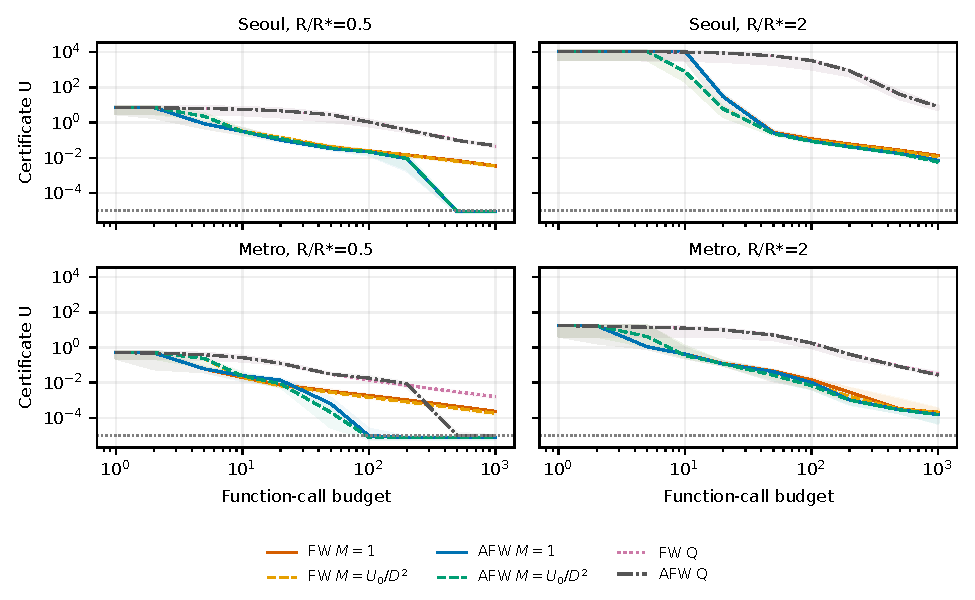
\includegraphics[width=\textwidth]{figures/additional_counts.pdf}
\caption{Additional real count datasets. Median certificate and
interquartile band over every signed coordinate vertex, at separate
function-call budgets. Completed runs are carried forward; nonterminal
runs reach the displayed budgets. BT has no curvature inputs; Q receives
analytic $H_0,H_1$. Radii and starts within a dataset share training data.}
\label{fig:multidata}
\end{figure}

\subsection{Auto-conditioned comparison on the additional count datasets}
We add 108 AC-FW runs to the same 108 Seoul/Metro cases, preserving the
648 earlier records. Algorithms 1--2 and Eq.~(6) with $\delta=1$
of~\cite{autoconditioned} are implemented independently, with the
mandatory initial vertex move and both initial source evaluations
charged. Rejected trials consume the 1000-outer-trial cap. Actual
counts are $N_f=N_{\rm LMO}=N+2$ and $N_g=N_{\rm accepted}+2$.
Parameter-hidden tests on both datasets instrument actual calls.

The common budget of 1000 function calls is reached by every
nonterminal run before its cap. AC-FW certifies 13/24 active Metro
starts, with median endpoint function count 385, and no start in the
other three dataset/radius conditions. FW-BT has 2/24 and 3/24
active Metro successes at this budget, while both AFW-BT variants
have 24/24. On active Seoul, AFW-BT has 30/30 and AC-FW has none.
All seven scalar-certificate variants remain unsuccessful on both
interior domains at 1000 function calls. These are oracle-budget
observations, not a uniform performance or runtime ranking.

The exponential objective is not globally gradient-Lipschitz on
$\R^d$, so this remains an empirical use on compact $Q$ rather than
a verbatim application of the cited global theorem. The new archive
contains 3240 budget prefixes and full-source audits. The focused
article joins these records with the six preserved methods in its
generated tables and vector figure.

\subsection{Paid causal certificate controls}
\label{sec:certificateexperiment}
We repeat the 432 BT trajectories from Section~\ref{sec:multidata},
using the same 108 dataset/radius/vertex cases and four methods. All
original terminal values, certificates, update counts and oracle counts
match the earlier archive exactly. The five controls are scalar,
disjoint blocks of $K=8,32,128$, and known $\mu=0.01$, as defined in
Section~\ref{sec:tangentmonitors}. Block sizes are fixed before observing
the results. These give 2160 dependent causal stopping profiles, not
2160 independent optimization runs. No new data or starting points
are introduced.

The monitors see only paid source values and gradients; neither the
line search nor initialization changes. We record the first causal
prefix with certificate at most $10^{-5}$, or the original endpoint.
Twenty native online-stop checks on a synthetic interior instance verify
the prefix construction and actual oracle costs for every method/profile
pair. Each profile's isolated LMO cost includes its own block
queries and the direction queries, excluding the other monitors.
An affordable budget prefix must pay the entire scheduled verification
at its source. No incomplete block is queried, and references are not
monitor inputs. The original trajectory cap is retained.

All three block sizes fail to produce any earlier stop: each retains
129/432 successes. At the common original endpoint, $K=8$ improves
the certificate on 61 paths and $K=32$ on 22, but the improvements do
not cross the tolerance. Blocks increase total LMO cost on 432, 425,
and 380 paths, respectively. This negative control does not establish
failure of other weights, block sizes, or exact Fenchel dual evaluation.

The known-$\mu$ control gives 226/432 successes and 110 earlier
prefixes without additional LMOs. On interior Metro all four methods
certify 24/24 starts. FW's function-call medians become 746.5 and
724.5, versus censored scalar medians 2000 and 2002; AFW's become
481.5 and 458, versus 2000 and 2001. At the separate budget of
1000 function calls, FW has 18/24 and 15/24 successes, and both AFW
variants have 24/24. Interior Seoul remains difficult: AFW has 4/30
and 10/30 successes at the full cap, but none at 1000 function calls;
FW has none. Active-regime success counts are unchanged.

Thus a standard certificate using analytical model information resolves
much of the observed Metro stopping lag, while the tested first-order
block controls do not. The known-$\mu$ result is not evidence of
adaptation to unknown strong convexity or a new rate. The original
scalar-certificate bounds remain the main analytical claim.
Full-path audits check lower-bound validity, certificate monotonicity,
dominance over scalar, and the exact extra-LMO schedule before sampling.
Active-set scans remain additional work; no wall-clock comparison is made.

\begin{table}[htbp]
\centering\small
\caption{Interior causal stopping controls. Each cell is the certified count and median function calls up to its first stop or the original cap; censored cases are included. Seoul has 30 starts per method, Metro 24. $F/A$: FW/AFW; subscripts $1,U$: initial $M=1,U_0/D^2$. Blocks use one additional full LMO per completed block; the known-$\mu$ column receives extra problem information.}
\label{tab:certificates}
\begin{tabular}{llrrrrr}
\hline
Data & Method & Scalar & $K=8$ & $K=32$ & $K=128$ & Known $\mu$ \\
\hline
Seoul & $F_1$ & 0; 2001 & 0; 2001 & 0; 2001 & 0; 2001 & 0; 2001 \\
Seoul & $F_U$ & 0; 1996 & 0; 1996 & 0; 1996 & 0; 1996 & 0; 1996 \\
Seoul & $A_1$ & 0; 2001 & 0; 2001 & 0; 2001 & 0; 2001 & 4; 2001 \\
Seoul & $A_U$ & 0; 1995.5 & 0; 1995.5 & 0; 1995.5 & 0; 1995.5 & 10; 1995 \\
\hline
Metro & $F_1$ & 0; 2000 & 0; 2000 & 0; 2000 & 0; 2000 & 24; 746.5 \\
Metro & $F_U$ & 0; 2002 & 0; 2002 & 0; 2002 & 0; 2002 & 24; 724.5 \\
Metro & $A_1$ & 6; 2000 & 6; 2000 & 6; 2000 & 6; 2000 & 24; 481.5 \\
Metro & $A_U$ & 7; 2001 & 7; 2001 & 7; 2001 & 7; 2001 & 24; 458 \\
\hline
\end{tabular}
\end{table}

\begin{figure}[htbp]
\centering
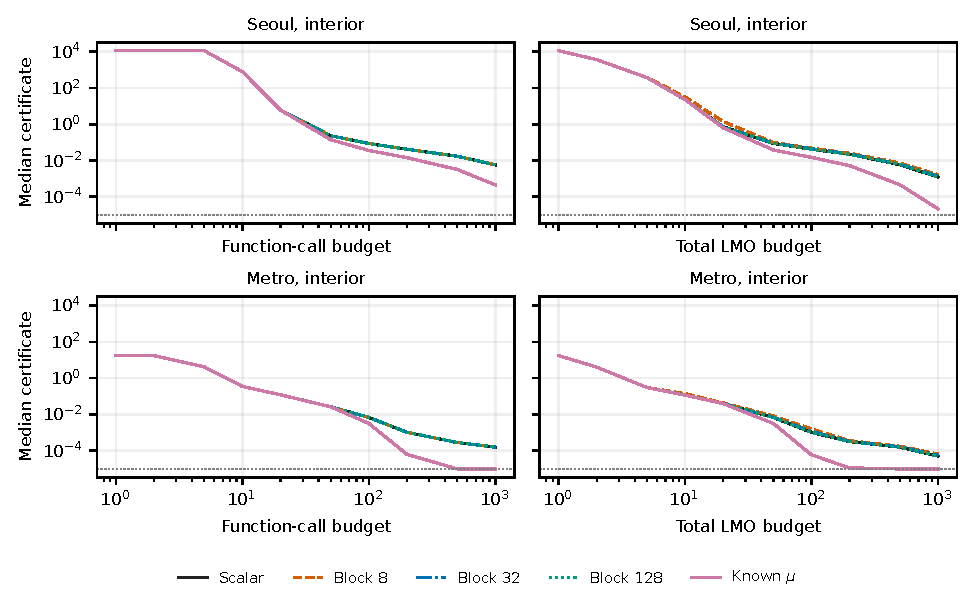
\includegraphics[width=\textwidth]{figures/causal_certificates.pdf}
\caption{Causal controls on interior AFW-BT paths with initial
$M=U_0/D^2$. Median certificates over all 30 Seoul or 24 Metro vertices
at separate function and total LMO budgets; total LMOs include the
profile's block queries. Completed prefixes are carried forward.
Known $\mu$ receives analytical ridge information; blocks do not.
All methods and both initializations appear in
Table~\ref{tab:certificates} and the archived report.}
\label{fig:causalcertificates}
\end{figure}


\section{Discussion}
The main candidate result is a two-phase certificate analysis of ordinary
quadratic backtracking without smoothness inputs, counting both LMO and all
function trials. Overestimated curvature requires only an additional
phase-controlled number of steps. Certificate normalization is optional:
the order alone does not justify it as a new algorithmic contribution.
The LMO guarantee also holds for the explicit rules and exact line search.
The empirical results support reporting unfavorable
regimes, controlling initialization, and separating oracle costs. On a
planted active family, the compulsory vertex move largely explains the
earlier apparent advantage of AC-FW over the chosen backtracking baselines.
Away steps provide a standard way to remove obstructing atoms without a
special initial move. Their established geometric progress inequality
also yields our phase bound under an additional geometric error bound.
The certificate conversion itself needs no strong convexity: feasible
descent provides a local gap envelope. Only the geometric error bound
is required separately in the logarithmic phase theorem.
The known linear convergence of AFW is not a novelty claim; the candidate
specialization concerns the separated curvature dependence, this stopping
certificate, and total trial cost.
The radius/units control also shows that fixed numerical curvature
initialization can affect outcomes on equivalent objectives; matching
the units of $M$ is necessary for an objective-scale comparison.
On the additional count datasets, success in active regimes does not
extend uniformly to larger interior domains. Independent reference
intervals expose a gap between primal accuracy and observable stopping.
The tested block tangent bounds do not improve stopping and add LMO cost.
A standard known-$\mu$ control improves Metro stopping without extra
LMOs, showing the role of available model information. Its residual
failures on Seoul limit a general claim. Neither control adds a new
duality or convergence result.

Open work includes a complete comparison with certificate/restart and
relative-smoothness analyses, an adaptive sliding baseline, independent
validation of the proof, more natural positive-$H_1$
applications, and pairwise extensions. Noisy directions and
finite-precision robustness require additional theory. Convexity of
the feasible region ensures that segment updates are feasible; a transfer
to an $\ell_0$ constraint does not follow from the present argument.

\appendix
\section{What direct substitutions into existing bounds establish}
\label{sec:prioranalysis}
This comparison concerns the stated bounds below, rather than every
consequence of the cited papers. It does not establish bibliographic priority.

Pedregosa et al.~\cite{pedregosa}, Theorem 3, give a convex primal--dual
bound in terms of averaged accepted smoothness estimates. Thus adaptive
curvature and last-iterate dual guarantees are already present there.
One cannot identify that dual value with the maximum of scalar tangent
lower bounds used here: their dual variable averages gradients. This
distinction alone does not prove a new rate; a transfer argument along
the algorithm's trajectory could still exist.

Here is an elementary illustration of the certificate distinction. For
$f(x)=x^2/2$ on $[-1,1]$, the scalar tangent lower bound is
$a(x)=-x^2/2-|x|$, whereas the Fenchel dual value is
$\psi(u)=-u^2/2-|u|$. For the history $(-1,1)$,
\[
 \max_i a(x_i)=-3/2 < \psi((x_0+x_1)/2)=0.
\]
For the history $(-1,-1/2)$,
\[
 \max_i a(x_i)=-5/8 > \psi(-3/4)=-33/32.
\]
Thus the two lower bounds have no universal ordering for arbitrary
tangent histories. These histories are not asserted to be iterates of
the cited algorithm; neither example contradicts its theorem.

A global Euclidean-smoothness substitution also loses information.
Let $\Delta_Q=\max_{x\in Q}(f(x)-f_Q^*)$. Assumption~\eqref{eq:curvature}
gives a valid bound $L_Q=H_0+H_1\Delta_Q$ on $Q$. Applying a conventional
$O(L_QD^2/\varepsilon)$ estimate retains $\Delta_Q/\varepsilon$, rather
than the logarithmic $H_1$ term. Replacing $\Delta_Q$ by $U_0$ is not
automatically valid: $U_0$ only bounds the initial suboptimality.
Restricting $Q$ to an initial sublevel set changes its LMO. Our local
acceptance argument avoids that restriction, followed by a phase-wise
count of estimates that remain too large. A finer use of an existing
average-curvature bound remains an open priority question.

The relative-smooth framework of Takahashi, Pokutta, and
Takeda~\cite{bregmanfw} uses a kernel, a segment scaling condition, and
additional assumptions for its accelerated conclusions. Its Euclidean
specialization recovers ordinary smoothness bounds, so choosing a
Euclidean kernel and $L=L_Q$ alone does not yield the separated
$H_0,H_1$ dependence above. This does not exclude a more suitable
kernel or a refined specialization of that analysis.

For adaptive sliding~\cite{adcgs}, Corollary 3.3 concerns outer
iterations with a running maximum of local curvature estimates;
Theorem 2.1 separately bounds inner LMO effort. Its restarted
Theorem 4.1 additionally assumes local strong convexity and uses local
smoothness and strong-convexity parameters in the restart schedule.
Our curvature assumption does not imply strong convexity: for example,
$f(x_1,x_2)=\cosh(x_1)-1$ on $[-1,1]^2$ has $H_0=H_1=1$ and a line
of minimizers. Consequently the restarted strong-convexity theorem
cannot be invoked from our assumptions alone. A complete comparison
must count all inner LMO calls and preserve the stopping certificate;
we do not establish superiority over sliding methods.

Wirth, Pe\~na, and Pokutta~\cite{wirth}, Definition 2.3(b) and
Theorem 3.6, use a uniform extended-curvature constant and a vertex
error bound for exact line search or a short step. Their linear
and two-regime rates are prior results. Directly substituting a
global $L_QD^2$ retains global curvature; a varying-curvature extension
would require further analysis.

Kerdreux, d'Aspremont, and Pokutta~\cite{restartfw}, Proposition 4.2
and Theorem 5.1, already combine burn-in, computable strong-Wolfe
stopping, unknown error-bound parameters, and cumulative LMO counts.
The stated bound uses global away curvature. Our phases analyze
ordinary backtracking without algorithmic restarts; this difference
does not itself establish a novel bound.

Zhao~\cite{zhao}, Theorems 4.1--4.2, establishes linear rates for both
objective error and FW gap with logarithmically homogeneous barriers.
Algorithm 1
uses exact search or a local-Hessian analytic step, rather than our
first-order quadratic backtracking. The function assumptions differ.
The passage from primal to gap rates is therefore also prior in
spirit, and is not claimed as novel here.


\begin{thebibliography}{99}
\bibitem{lacoste2016} S.~Lacoste-Julien.
Convergence Rate of Frank-Wolfe for Non-Convex Objectives.
\href{https://arxiv.org/abs/1607.00345}{arXiv:1607.00345}, 2016.
\bibitem{wirth} E.~Wirth, J.~Pe\~na, and S.~Pokutta.
Fast convergence of Frank-Wolfe algorithms on polytopes.
\href{https://arxiv.org/abs/2406.18789v3}{arXiv:2406.18789v3}, 2025.
\bibitem{restartfw} T.~Kerdreux, A.~d'Aspremont, and S.~Pokutta.
Restarting Frank-Wolfe: Faster Rates under H\"olderian Error Bounds.
\href{https://arxiv.org/abs/1810.02429v4}{arXiv:1810.02429v4}, 2021.
\bibitem{zhao} R.~Zhao.
New Analysis of an Away-Step Frank-Wolfe Method for Minimizing
Logarithmically-Homogeneous Barriers.
\href{https://arxiv.org/html/2305.17808v4}{arXiv:2305.17808v4}, 2023.
\bibitem{lacostejaggi} S.~Lacoste-Julien and M.~Jaggi.
On the Global Linear Convergence of Frank-Wolfe Optimization Variants.
\emph{NeurIPS}, 2015.
\href{https://arxiv.org/abs/1511.05932}{arXiv:1511.05932}.
\bibitem{warmup} F.~Alimisis, R.~Islamov, and A.~Lucchi.
Why Do We Need Warm-up? A Theoretical Perspective.
\href{https://arxiv.org/abs/2510.03164v2}{arXiv:2510.03164v2}, 2026.
\bibitem{vyguzov} A.~A.~Vyguzov and F.~S.~Stonyakin.
Frank-Wolfe Algorithms for $(L_0,L_1)$-smooth functions.
\href{https://arxiv.org/abs/2510.16468v5}{arXiv:2510.16468v5}, 2026.
\bibitem{lobanov} A.~Lobanov.
A Few Accelerated Algorithms for Convex Optimization under $(H_0,H_1)$-Smoothness.
\href{https://arxiv.org/abs/2608.04884}{arXiv:2608.04884}, 2026.
\bibitem{lobanovkoloskova} A.~Lobanov and A.~Koloskova.
Avoiding Bias in Clipped SGD for Overparameterized Models under Generalized Smoothness.
\href{https://arxiv.org/abs/2605.14800v2}{arXiv:2605.14800v2}, 2026.
\bibitem{braun} G.~Braun, A.~Carderera, C.~W.~Combettes, H.~Hassani,
A.~Karbasi, A.~Mokhtari, and S.~Pokutta. Conditional Gradient Methods.
\href{https://arxiv.org/abs/2211.14103v5}{arXiv:2211.14103v5}, 2025.
\bibitem{pedregosa} F.~Pedregosa, G.~Negiar, A.~Askari, and M.~Jaggi.
Linearly Convergent Frank-Wolfe with Backtracking Line-Search.
\emph{AISTATS}, 2020. \href{https://arxiv.org/abs/1806.05123}{arXiv:1806.05123}.
\bibitem{karimi} H.~Karimi, J.~Nutini, and M.~Schmidt.
Linear Convergence of Gradient and Proximal-Gradient Methods Under the
Polyak--{\L}ojasiewicz Condition.
\href{https://arxiv.org/abs/1608.04636v4}{arXiv:1608.04636v4}, 2020.
\bibitem{hendrych} D.~Hendrych, M.~Besan\c{c}on, D.~Mart\'inez-Rubio, and S.~Pokutta.
Secant Line Search for Frank-Wolfe Algorithms.
\href{https://arxiv.org/abs/2501.18775v2}{arXiv:2501.18775v2}, 2025.
\bibitem{selfconcordant} P.~Dvurechensky, K.~Safin, S.~Shtern, and M.~Staudigl.
Generalized Self-Concordant Analysis of Frank-Wolfe Algorithms.
\href{https://arxiv.org/abs/2010.01009}{arXiv:2010.01009}, 2020.
\bibitem{wdbc} W.~Wolberg, O.~Mangasarian, N.~Street, and W.~Street.
Breast Cancer Wisconsin (Diagnostic) [Dataset]. UCI Machine Learning Repository, 1993.
\href{https://doi.org/10.24432/C5DW2B}{doi:10.24432/C5DW2B}.
\bibitem{autoconditioned} K.-H.~Giang-Tran, S.~Shafiee, and N.~Ho-Nguyen.
Auto-Conditioned Frank-Wolfe Algorithms.
\href{https://arxiv.org/abs/2605.15512}{arXiv:2605.15512}, 2026.
\bibitem{bike} H.~Fanaee-T. Bike Sharing [Dataset]. UCI Machine Learning Repository, 2013.
\href{https://doi.org/10.24432/C5W894}{doi:10.24432/C5W894}. CC BY 4.0.
\bibitem{seoul} Seoul Bike Sharing Demand [Dataset].
UCI Machine Learning Repository, 2020.
\href{https://doi.org/10.24432/C5F62R}{doi:10.24432/C5F62R}. CC BY 4.0.
\bibitem{metro} J.~Hogue. Metro Interstate Traffic Volume [Dataset].
UCI Machine Learning Repository, 2019.
\href{https://doi.org/10.24432/C5X60B}{doi:10.24432/C5X60B}. CC BY 4.0.
\bibitem{bregmanfw} S.~Takahashi, S.~Pokutta, and A.~Takeda.
Fast Frank--Wolfe Algorithms with Adaptive Bregman Step-Size for Weakly Convex Functions.
\emph{ICLR}, 2026.
\href{https://arxiv.org/abs/2504.04330v4}{arXiv:2504.04330v4}.
\bibitem{adcgs} S.~Takahashi.
Adaptive Conditional Gradient Sliding: Projection-Free and Line-Search-Free Acceleration.
\href{https://arxiv.org/abs/2601.20443v2}{arXiv:2601.20443v2}, 2026.
\end{thebibliography}
\end{document}
